%%This is a very basic article template.
%%There is just one section and two subsections.
\documentclass{beamer}

\usepackage{calc,verbatim,amsmath,dsfont,subfig,setspace,varwidth}
%\usepackage{media9}
\usepackage{amsmath}
\newcommand{\data}{\mathcal{D}}
\newcommand{\given}{\mid}
\newcommand{\E}{\ensuremath{\mathds{E}}}
\newcommand{\thetas}{\boldsymbol{\theta}}

\usepackage{fontawesome}
\usepackage{graphicx}

\newcommand{\pros}{\item[\textcolor{green!80!black}\faThumbsOUp]}
\newcommand{\cons}{\item[\textcolor{red!80!black}\faThumbsODown]}

% Setup appearance:

\usetheme{Frankfurt}

\usefonttheme[onlylarge]{structurebold}
\setbeamerfont*{frametitle}{size=\normalsize,series=\bfseries}
\setbeamertemplate{navigation symbols}{}

\definecolor{ubcblue}{RGB}{0,40,89}
\definecolor{ubcgray}{RGB}{116,145,163}

\setbeamercolor{section in toc}{fg=ubcblue,bg=white}
\setbeamercolor{alerted text}{fg=ubcblue}
\setbeamercolor*{palette primary}{fg=white,bg=ubcblue}
\setbeamercolor*{palette secondary}{fg=ubcblue,bg=ubcblue}
\setbeamercolor*{palette tertiary}{fg=white,bg=ubcblue}
\setbeamercolor*{palette quaternary}{fg=ubcgray!50!white,bg=ubcblue}

\setbeamercolor{item projected}{bg=ubcblue,fg=white}
\setbeamercolor{block title}{bg=ubcgray}
\setbeamercolor{block body}{bg=ubcgray!20!white}
\setbeamercolor{description item}{fg=ubcblue}
\setbeamercolor{caption name}{fg=ubcblue}

\setbeamerfont*{frametitle}{size=\Large}
\setbeamerfont*{title}{size=\Large}
\setbeamerfont*{section in toc}{size=\large}
\setbeamerfont*{block title}{}
\setbeamerfont*{item projected}{size=\footnotesize}
\setbeamerfont*{alerted text}{series=\bfseries}

\usepackage[english]{babel}
\usepackage[latin1]{inputenc}
\usepackage{animate}

\usepackage{times}
\renewcommand*\sfdefault{uop}

\usepackage[T1]{fontenc}

\usepackage[vlined]{algorithm2e}
\SetNlSty{}{}{}
\SetArgSty{}
\DontPrintSemicolon

% Setup TikZ

\usepackage{tikz,pgfplots,siunitx,xfrac,comment,booktabs,etoolbox,multirow}
\robustify\bfseries
\newcommand{\minitab}[2][l]{\begin{tabular}{@{}#1@{}}#2\end{tabular}}

\sisetup{
  seperr,
  %repeatunits=false,
  product-units = single,
  trapambigerr=false,
  trapambigrange=false,
  %tophrase={{ bis }},
  valuemode=math,
  unitmode=math,
  quotient-mode=fraction,
  fraction-function=\sfrac
}

\usetikzlibrary{arrows,fadings,fit,positioning,spy,shapes.geometric}
\usetikzlibrary{matrix,shadows,decorations,backgrounds,scopes}
\usetikzlibrary{intersections,3d,calc,decorations.pathreplacing}

\pgfdeclarelayer{background}
\pgfsetlayers{background,main}
%\pgfplotsset{every extra y tick/.append style={grid style=black}}

\newcounter{slidenumber}
\newcounter{pagesofcurrentframe}
\newlength{\slidenumberwidth}

\setbeamertemplate{footline}{
\setcounter{slidenumber}{\insertpagenumber}%
\addtocounter{slidenumber}{-\insertframestartpage}%
\addtocounter{slidenumber}{1}%
\setcounter{pagesofcurrentframe}{\insertframeendpage}
\addtocounter{pagesofcurrentframe}{-\insertframestartpage}
\addtocounter{pagesofcurrentframe}{1}
\normalfont 
\leavevmode
\hbox{
\begin{beamercolorbox}[wd=.98\paperwidth,ht=2.5ex,dp=2.125ex,leftskip=.3cm,rightskip=.3cm]{title in head/foot_}
\insertauthor
\hfill 
\insertshorttitle
\hfill
\settowidth{\slidenumberwidth}{\inserttotalframenumber}
\ifnum\value{pagesofcurrentframe}>1
\tikz[baseline=(char.base)] {
	\node[inner sep=0pt, text width=\slidenumberwidth,align=right] (char)
   	{\insertframenumber};
}%
\tikz[baseline=(char.base)] {
	\node[inner sep=0pt, text width=1em,align=left] (char)
   	{\alph{slidenumber}};
}
\else
\tikz[baseline=(char.base)] {
	\node[inner sep=0pt, text width=\slidenumberwidth,align=right] (char)
   	{\insertframenumber};
}%
\tikz[baseline=(char.base)] {
	\node[inner sep=0pt, text width=1em,align=left] (char)
   	{};
}
\fi
  \end{beamercolorbox}
}
}

\newcommand{\vect}[1]{\mathbf{#1}}

\newcommand{\watermarklogo}{\includegraphics[width=4.5cm]{images/ubcblue.png}}

\usebackgroundtemplate{
\parbox[b][\paperheight+1.75cm]{\paperwidth+1cm}{
	\hfill\tikz 
	\node {\watermarklogo}
	node[fill=white,path fading=south,fading angle=45] {\phantom{\watermarklogo}}%
	node[fill=white,opacity=0.76] {\phantom{\watermarklogo}};
}
}

\newenvironment{questionmarks}{%
\usebackgroundtemplate{\parbox[b][%
\paperheight+1.45cm%
]{%
\paperwidth+1.45cm%
}{%
\hfill\tikz% 
\node {\includegraphics[width=0.55\textwidth]{images/ubcquestions.png}}% 
node[fill=white,path fading=south,fading angle=45]%
{\phantom{\includegraphics[width=0.55\textwidth]{images/ubcquestions.png}}}%
node[fill=white,opacity=0.3]%
{\phantom{\includegraphics[width=0.55\textwidth]{images/ubcquestions.png}}}; }}%
}{%
\usebackgroundtemplate{%
\parbox[b][\paperheight+1.75cm]{\paperwidth+1cm}{%
	\hfill\tikz %
	\node {\watermarklogo}%
	node[fill=white,path fading=south,fading angle=45] {\phantom{\watermarklogo}}%
	node[fill=white,opacity=0.76] {\phantom{\watermarklogo}};%
}%
}%
}

\newcommand{\footlineextra}[1]{
\begin{tikzpicture}[remember picture,overlay]
    \node[xshift=-1.5em,yshift=1em,anchor=south east] at (current page.south
    east) {\footnotesize #1};
\end{tikzpicture}
}

\tikzstyle{simplenode}=[shape=circle,draw=black,
top color=ubcgray!5,bottom color=ubcgray!40,
semithick]
\tikzstyle{basicnode}=[simplenode,circular drop shadow]

\title[Efficient Deep Learning for Manifold Learning and Lesion
Segmentation]{Efficient Deep Learning of 3D Structural Brain MRIs for Manifold
Learning and Lesion Segmentation with Application to MS}

\author{Tom Brosch}

\institute[Universities of British Columbia]
{
UBC MS/MRI Research Group\\
Electrical and Computer Engineering\\
University of British Columbia
}

\date{PhD Defence}
%\date{February 22, 2016}

\begin{document}

\begin{frame}
\titlepage
\end{frame}

\makeatletter
\setbeamertemplate{enumerate items}{
    \llap{\begin{pgfpicture}{-1ex}{-0.8ex}{1ex}{1ex}
      {\pgftransformscale{0.9}\pgftext{\beamer@usesphere{section number
      projected}{tocsphere}}} \pgftext{%
        \usebeamerfont*{section number projected}%
        \usebeamercolor{section number projected}%
        \color{fg!90!bg}%
        \insertenumlabel}
    \end{pgfpicture}%
    %\kern0.15ex
    }%
}
\makeatother

\begin{frame}{Outline}
\tableofcontents
\end{frame}

\section{Introduction}

\subsection*{Motivation}

\begin{frame}{Multiple Sclerosis}

%\begin{figure}[tb]
\centering
\begin{tikzpicture}
\tikzstyle{every node}=[font=\small]

\node[] (healthy)
{\includegraphics[width=0.5\textwidth]{images/healthyneuron}};
\node[,below=-.5cm of healthy] (damaged)
{\includegraphics[width=0.5\textwidth]{images/damagedneuron}};

\node[fit=(healthy)(damaged), inner sep=0] (neurons) {};

\node[right=1cm of neurons] (brain)
{\includegraphics[width=0.4\textwidth]{images/brain}};

\coordinate (m1) at (-0.75,0.9);
\coordinate (m2) at (0.95,0.9);
\coordinate (m3) at (1.65,-2.75);

\node[fit=(m1)(m2)] (myelin) {};

\node[above=0.65cm of myelin] (sheaths) {Myelin sheaths};

\draw (m1)--(sheaths);
\draw (m2)--(sheaths);

\node[ellipse,draw=red,thick,minimum width=1.3cm, minimum height=0.7cm,
label=90:Damaged myelin] at (m3) {};

\coordinate (wm) at (5.4,-0.5);
\coordinate (wml) at (5.3,-1.9);

%\draw[red] (wm) circle (3pt);
%\draw[red] (wml) circle (3pt);

\draw[gray,thick] (wm)--(healthy);
\draw[gray,thick] (wml)--(damaged);

%\draw[step=1cm,gray,very thin] (-1,2) grid (6,-4);

\end{tikzpicture}

% \caption[Demyelination in MS]{Due to the break down of the blood brain barrier,
% the bodies own immune system attacks the myelin sheaths of the axons, which
% causes the formation of demyelinating lesions, visible primarily in the white
% matter on conventional \gls{mri} scans. Lesions are highlighted in white.}
% \label{fig:ms}
% \end{figure}

\end{frame}

\begin{frame}{Multiple Sclerosis}
% Measure what is measurable, and make measurable what is not so.
\begin{itemize}
\item MS is a very heterogeneous disease
\item MS lesions vary greatly in number, size, and location
\item<2> MS also shows varying degrees of atrophy, most visible by an
enlargement of the ventricles
\end{itemize}
\begin{center}
\only<1>{%
\includegraphics[height=0.35\textwidth]{images/fewlesions}\quad
\includegraphics[height=0.35\textwidth]{images/manylesions}\quad
\includegraphics[height=0.35\textwidth]{images/periventricular}%
}%
\only<2>{%
\includegraphics[height=0.35\textwidth]{images/lowatrophy3}\quad
\includegraphics[height=0.35\textwidth]{images/mediumatrophy}\quad
\includegraphics[height=0.35\textwidth]{images/highatrophy}%
}
\end{center}
\end{frame}

\begin{frame}{Motivation and Challenges}
Clinical motivation:
\begin{itemize}
\item \alert{To measure disease state and progression}
\item To automatically and accurately segmented MS lesions in order to derive
lesion-based biomarkers such as lesion volume and lesion count
\item To develop a method that can automatically discover patterns of
variability in brain morphology and lesion distribution
\end{itemize}
\vspace{0.5em}
Challenges:
\begin{itemize}
\item Large anatomical and pathological variability
\item Large variability in contrasts produced by different scanners
\item Patterns of morphological variability and lesion
distribution are highly nonlinear 
\end{itemize}
\end{frame}

\begin{comment}

\subsection{Related Work}

\begin{frame}{Related Work: Lesion Segmentation /1}
Unsupervised methods:
\begin{itemize}
\item Segmentation based on a per-subject per-image model
\item Lesion voxels are modelled as an outlier of the intensity distribution of
normal tissue or a separate intensity cluster
\pros Robust to inter-subject and inter-image variability
\cons Sensitive to non-lesion outliers such as blood vessels and partial volume
effects
\end{itemize}
\pause
\vspace{0.5em}
Supervised methods:
\begin{itemize}
\item Segmentation as a voxel classification problem
\item Vary by used features and classification algorithm
\pros Lesion-specific
\cons Sensitive to inter-subject and inter-scanner variability
\end{itemize}
\end{frame}

\begin{frame}{Related Work: Lesion Segmentation /2}
End-to-end learning:
\begin{itemize}
\item Joint learning of features and classifier from labelled data
using a convolutional neural network (CNN)
\item Classify image patches using a CNN (patch-based)
\item Feed in entire volumes into a CNN (fully convolutional)
%\pros<2-> Lesion-specific
\vspace{0.5em}
\pros Learning of features that are tuned to the data and segmentation task
\pros Can learn features that are robust to inter-subject and inter-scanner
variability
\cons Requires large amounts of training data
\cons Training and inference of patch-based approaches can be prohibitively
slow
\end{itemize}
\end{frame}

\begin{frame}{Related Work: Manifold Learning}
\end{frame}

\end{comment}

% \begin{frame}{Objectives and Challenges}
% \begin{block}{Objective}
% To investigate the use of deep learning methods for medical image analysis.
% \end{block}
% 
% Common properties of deep learning methods:
% \begin{itemize}
% \item The use of multiple layers of nonlinear processing units for feature
% extraction
% \item Layers are organized to form a hierarchy of low-level to high-level
% features
% \pros Can learn features that are robust to large variability
% \pros Can automatically discover highly nonlinear patterns of variability in
% groups of images
% \end{itemize}
% %\vspace{0.5em}
% Challenges for medical image analysis:
% \begin{itemize}
% \item Memory requirements to store high-resolution 3D images
% \item Calculation of 3D convolutions computationally demanding
% \end{itemize}
% \end{frame}

\subsection*{Objectives}

% first point important for MS lesion segmentation
% Second point motivates the use for manifold learning

\begin{frame}{Objectives}
\begin{block}{Objectives}
To develop deep learning methods for neuroimage analysis and to measure their
performance.
\end{block}
\vspace{0.5em}
Motivation:
\begin{itemize}
\item Can learn features that are robust to large variability
\item Can discover highly nonlinear patterns of variability
\end{itemize}
\vspace{0.5em}
Technical challenges:
\begin{itemize}
\item Relatively small size of medical data sets
\item High dimensionality of 3D medical images
\end{itemize}
\end{frame}

\begin{frame}{Contributions}
\begin{itemize}
\item Developed a computation and memory efficient training algorithm for
convolutional deep learning models
\vspace{0.5em}
\item Developed a novel segmentation method that learns features at
different scales that are tuned to a given combination of image types and
segmentation task
\item Proposed a novel objective function for neural networks that facilitates
the training on vastly unbalanced training sets
\vspace{0.5em}
\item First work to demonstrate the use of deep learning for manifold learning
of 3D medical images
\item Developed a framework for modelling changes in brain morphology and lesion
distribution
\end{itemize}
\end{frame}

\section[Deep Learning in the Frequency Domain]{Efficient Deep Learning in the
Frequency Domain}

\subsection{Training Algorithm}

\begin{frame}{Introduction to Deep Learning}

\begin{columns}[onlytextwidth]
\begin{column}{0.53\textwidth}
\centering
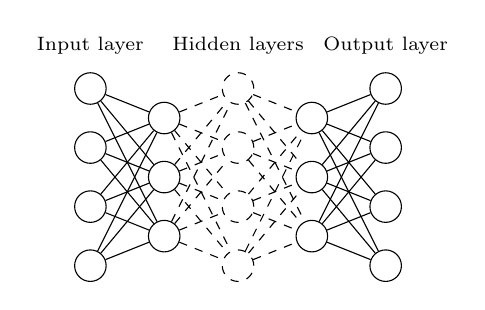
\begin{tikzpicture}[scale=0.75]
\tikzstyle{aenode}=[circle,draw,minimum width=0.4cm]
\tikzstyle{gnode}=[circle,draw,minimum width=0.4cm,dashed]
\tikzstyle{every node}=[font=\scriptsize]

\foreach \y in {1,...,4} {
  \node[aenode] (inode\y) at (0, \y) {};
}

\begin{scope}[yshift=0.5cm]
\foreach \y in {1,...,3} {
  \node[aenode] (h1node\y) at (1.25, \y) {};
}
\end{scope}

\foreach \y in {1,...,4} {
  \node[gnode] (h2node\y) at (2.5, \y) {};
}

\begin{scope}[yshift=0.5cm]
\foreach \y in {1,...,3} {
  \node[aenode] (h3node\y) at (3.75, \y) {};
}
\end{scope}

\foreach \y in {1,...,4} {
  \node[aenode] (onode\y) at (5, \y) {};
}


\foreach \x in {1,...,4} {
  \foreach \y in {1,...,3} {
    \draw[-] (inode\x)--(h1node\y);
    \draw[-,dashed] (h1node\y)--(h2node\x);
    \draw[-,dashed] (h2node\x)--(h3node\y);
    \draw[-] (h3node\y)--(onode\x);
  }
}

\node[above=3pt of inode4] {Input layer};
%\node[above=3pt of h1node3] {$\vect{x}_1$};
\node[above=3pt of h2node4] (xl) {Hidden layers};
%\node[above=3pt of h3node3] {$\vect{x}_{L-1}$};
\node[above=3pt of onode4] {Output layer};

% \node[above=3pt of inode4] {$\vect{x}_0$};
% \node[above=3pt of h1node3] {$\vect{x}_1$};
% \node[above=3pt of h2node4] (xl) {$\vect{x}_l$};
% \node[above=3pt of h3node3] {$\vect{x}_{L-1}$};
% \node[above=3pt of onode4] {$\vect{x}_L$};
% 
% \path (h1node3)--node[above=2pt] {$\vect{W}_l$} (h2node4);

%\node[below=5pt of h2node1] (hiddens) {Hidden units};
%\node at (hiddens-|inode1) {Input units};
%\node at (hiddens-|onode1) {Output units};

\end{tikzpicture}

\end{column}
\begin{column}{0.47\textwidth}
%\only<1-3>{%
\begin{itemize}
\item Multiple layers of nonlinear processing units for feature extraction
\item Hierarchy of low-level to high-level features 
\end{itemize}%
%}%
% \only<2>{%
% \begin{itemize}
% \item Forward pass: Output prediction
% \item Backward pass: Error backpropagation
% \end{itemize}%
% }%
% \only<3>{%
% \begin{itemize}
% \item Forward pass: Feature extraction
% \item Backward pass: Image reconstruction
% \end{itemize}%
% }%
\end{column}
\end{columns}
\vspace{1.5em}
\centering
% \only<1>{%
% \begin{tabular}{@{}p{0.46\textwidth}p{0.46\textwidth}@{}}
% \toprule
% Neural Networks & Deep Belief Networks \\
% \midrule
% \\
% \\
% \\
% \\
% \bottomrule
% \end{tabular}
% }%
% \only<2>{%
% \begin{tabular}{@{}p{0.46\textwidth}p{0.46\textwidth}@{}}
% \toprule
% Neural Networks & Deep Belief Networks \\
% \midrule
% Supervised & \\
% Computational graph & \\
% Function approximation & \\
% Minimize the prediction error & \\
% \bottomrule
% \end{tabular}
% }%
%\only<3>
\footlineextra{[Werbos, 1974; Hinton et al., 2006]}
\end{frame}

\begin{comment}
\begin{frame}{Training of Convolutional Models}
\begin{center}
\begin{tikzpicture}

\tikzstyle{neuron}=[draw,circle,minimum width=0.6cm]
\tikzstyle{every node}=[font=\small]
\tikzstyle{every label}=[align=center,font=\small]
\tikzstyle{every pin}=[align=center,font=\small,overlay]
\tikzstyle{every pin edge}=[overlay]

\foreach \x in {0, 1, 2, 3} {
  \ifnum\x=3
  \node<1-2>[neuron] (input\x) at (0, \x) {};
  \node<3->[neuron,pin=180:3D image] (input\x) at (0, \x) {};
  \else
  \node[neuron] (input\x) at (0, \x) {};
  \fi
  \node[neuron] (hidden\x) at (2, \x) {};
}

\node<3>[neuron,thick,red!80] at (0, 3) {};

\node[neuron,dashed] (output) at (4, 1.5) {};

\node<1>[fit=(input0)(input3),draw,rounded corners=4pt, dashed,label=90:Input
layer\\$x^{(0)}$] {};

\node<2>[fit=(input0)(input3),draw,rounded corners=4pt,label=90:Input
layer\\$x^{(0)}$,thick,red!80,pin=180:Multichannel\\image] {};

\node<3->[fit=(input0)(input3),draw,rounded corners=4pt,label=90:Input
layer\\$x^{(0)}$,dashed,pin=180:Multichannel\\image] {};

\node[fit=(hidden0)(hidden3),draw,rounded corners=4pt, dashed,label=90:Hidden
layer\\$x^{(l)}$] {};

% \node[fit=(output),draw,rounded corners=4pt, dashed,label=90:Output
% layer\\$x^{(L)}$] {};

\foreach \x in {0, 1, 2, 3} {
  \foreach \y in {0, 1, 2, 3} {
    \draw (input\x)--(hidden\y);
  }
  \draw[dashed] (hidden\x)--(output);
}

\only<4>{
  \draw[thick,red!80] (input3)--(hidden3);
}

\only<4->{
  \path (input3)--node[above,font=\small]{$*\tilde{w}^{(l)}_{ij}$} (hidden3);
}

% \only<5>{
%   \foreach \x in {0, 1, 2, 3} {
%     \draw[thick,red!80] (input\x)--(hidden3);
%   }
% }
% 
% \only<5->{
% \path (input3)--
%   node[above, align=center, font=\small]{Multichannel\\ filter kernel}
%   (hidden3);
% }

\end{tikzpicture}
\end{center}
\uncover<5>{
\begin{block}{Activations of a convolutional layer}
\vspace*{-1em}
\begin{align*}
x^{(l)}_j &= f\Big(\sum_i \tilde{w}^{(l)}_{ij}*x^{(l-1)}_i\Big) & \text{for }l
\in [1,L]
\end{align*}
\end{block}
}
\end{frame}
\end{comment}

% TODO: Introduce convolutional model
% Why? When applied to high-resolution images, number of weights increases
% quadratically with the number of voxels
% Convolutional model: nodes are images, connections are convolutions
% Greatly reduces the number of trainable parameters, because now one unit per
% channel and not per voxel

\begin{frame}{Introduction to Deep Learning}
Fully connected models:
\begin{itemize}
\item Number of weights increases quadratically with the number of voxels
\item Number of trainable weights too high for application to 3D
volumes
\end{itemize}
\vspace{0.5em}
Convolutional models:
\begin{itemize}
\item Number of weights greatly reduced due to local connectivity and weight
sharing
\item Strided convolutions further reduce the number of hidden units
\item Scale much more efficiently with image resolution
\item Calculation of convolutions computationally demanding 
\end{itemize}
\footlineextra{[LeCun et al., 1998]}
\end{frame}

\begin{frame}{Training of Convolutional Models}
\begin{block}{Observation}
The computational bottleneck is the calculation of $O(NFC)$ convolutions.
% , where
% $N$ is the number of images, $F$ is the number of convolutional filter kernels,
% and $C$ is the number of channels per image.
\end{block}
\vspace{0.5em}
Approach 1: Na\"ive FFT-based implementation
\begin{itemize}
\item Replaces convolutions with FFTs and element-wise multiplications
\item Requires $O(NFC)$ FFT calculations
\end{itemize}
\vspace{0.5em}
Approach 2: Training in the Frequency Domain
\begin{itemize}
\item Maps all operations to frequency domain, when possible
\item Only calculates operations in spatial domain that cannot be calculated in
the frequency domain
\item Requires $O(NC + FC + NF)$ FFT calculations
\end{itemize}
\footlineextra{[Brosch and Tam, Neural Computation, 2015]}
\end{frame}

% Some mappings are obvious such as the scalar multiplication and element-wise
% addition. Key to the success of the method was that we also found a way to
% express flipping of a convolutional kernel and to express strided convolutions
% as stride-1 convolutions

% TODO: Training slide
% Bottleneck is the calculation of convolutions
% Approach 1: Naive FFT implementation
% Map convolutions to element-wise multiplications
% Requires O(NFC) number of FFTs
% Approach 2: Perform training in the frequency domain
% Only go to spatial domain for operations that cannot be performed in the
% frequency domain
% O(NF+FC+NC) FFTs

\begin{comment}

\begin{frame}{Training of Convolutional Models}
\begin{itemize}
\item Show same graph as before
\item Units are 3D images
\item Relationships between units are expressed in terms of convolutions
\item Neural network: estimating the error and error backpropagation (show with
arrows)
\item Deep belief network: Generating data-dependent and data-independent
samples required to estimate the gradient using a Monte Carlo approach (show
with arrows)
\item Computational bottleneck is the calculation of convolutions
\end{itemize}
\end{frame}

\newcommand*\pannotate[3]{%
\tikz[baseline=(char.base)] {
  \node[inner sep=0] (char) {#1};
  \only<2>{
  \node[fit=(char),draw=red,thick,overlay,ellipse,inner sep=2pt,
  pin={[overlay,pin edge={-,overlay}]#2:#3}] {};}
}}

\newcommand*\lannotate[3]{%
\tikz[baseline=(char.base)] {
  \node[inner sep=0] (char) {#1};
  \only<2>{
  \node[fit=(char),draw=red,thick,overlay,ellipse,inner sep=2pt,
  label={[overlay]#2:#3}] {};}
}}

\begin{frame}{Training in the Spatial Domain}
\tikzstyle{na} = [baseline=-.5ex,remember picture]
\footnotesize
\begin{columns}[t]
\begin{column}{0.7\textwidth}
\emph{Spatial domain}
\begin{algorithm}[H]
\setstretch{1.15}
Initialize\;
\ForEach{image $v \in \data$} {
  \tcp{Forward pass}
  \ForEach{filter $j$} {
    $h_j = 0$\;
    \ForEach{channel $i$} {
      $h_j = h_j$\,$+$\,\pannotate{$\tilde{w}_{ij} * v_i$}{30}{$N\times F\times
      C$}\; }
    $h_j = f(h_j)$\;
  }
  \tcp{Backward pass}
  \ForEach{channel $i$} {
    $v_i = 0$\;
    \ForEach{filter $j$} {
      $v_i = v_i$\,$+$\,\pannotate{$w_{ij} \circledast h_j$}{30}{$N\times
      F\times C$}\; }
    $v_i = f(v_i)$\;
  }
}
\end{algorithm}
\end{column}
\begin{column}{0.3\textwidth}
\emph{Frequency domain}
\end{column}
\end{columns}
\end{frame}

\begin{frame}{Training using FFTs}
\tikzstyle{na} = [baseline=-.5ex,remember picture]
\footnotesize
\begin{columns}[t]
\begin{column}{0.7\textwidth}
\tikz \coordinate (right) at (0.6\textwidth, 0);%
\emph{Spatial domain}
\begin{algorithm}[H]
\setstretch{1.15}
Initialize\;
\ForEach{image $v \in \data$} {
  \tcp{Forward pass}
  \ForEach{filter $j$} {
    $h_j = 0$\;
    \ForEach{channel $i$} {
      $h_j = h_j + z$\tikz[na] \coordinate (first) at (1,0);\;
    }
    $h_j = f(h_j)$\;
  }
  \tcp{Backward pass}
  \ForEach{channel $i$} {
    $v_i = 0$\;
    \ForEach{filter $j$} {
      $v_i = v_i + z$\tikz[na] \coordinate (second) at (1,0);\;
    }
    $v_i = f(v_i)$\;
  }
}
\end{algorithm}
\end{column}
\begin{column}{0.3\textwidth}
\emph{Frequency domain}\\
\begin{tikzpicture}[overlay,remember picture]

\coordinate (left);

% Forward
% \draw[->, shorten >=10pt, shorten <=10pt] ([yshift=2pt]first-|right) --
%   node[above]{$\hat{v}_i$\,$=$\,
%   \lannotate{$\mathcal{F}(v_i)$}{90}{$N\times F\times C$},
%   $\hat{w}_{ij}$\,$=$\,
%   \lannotate{$\mathcal{F}(\tilde{w}_{ij})$}{90}{$N\times F\times C$}}
%   ([yshift=2pt]first-|left);
% 
% \draw[<-, shorten >=10pt, shorten <=10pt] ([yshift=-2pt]first-|right) --
%   node[below]{$z$\,$=$\,
%   \lannotate{$\mathcal{F}^{-1}(\hat{z})$}{-90}{$N\times F\times C$}}
%   ([yshift=-2pt]first-|left);

\draw[->, shorten >=10pt, shorten <=10pt] ([yshift=2pt]first-|right) --
  node[above] (f1) {$\hat{v}_i=\mathcal{F}(v_i),
  \hat{w}_{ij}=\mathcal{F}(\tilde{w}_{ij})$}
  ([yshift=2pt]first-|left);

\draw[<-, shorten >=10pt, shorten <=10pt] ([yshift=-2pt]first-|right) --
  node[below] (f2) {$z=\mathcal{F}^{-1}(\hat{z})$}
  ([yshift=-2pt]first-|left);
  
\node<2>[fit=(f1)(f2),inner sep=-3pt,ellipse,draw=red,thick,pin={90:$N \times
F\times C$}] {};

\node[right] at (left|-first) {$\hat{z} = \hat{w}_{ij} \cdot \hat{v}_i$};

% Backward
\draw[->, shorten >=10pt, shorten <=10pt] ([yshift=2pt]second-|right) --
  node[above] (b1) {$\hat{h}_j=\mathcal{F}(h_j),
  \hat{w}_{ij}=\mathcal{F}(w_{ij})$} ([yshift=2pt]second-|left);

\draw[<-, shorten >=10pt, shorten <=10pt] ([yshift=-2pt]second-|right) --
  node[below] (b2) {$z=\mathcal{F}^{-1}(\hat{z})$}
  ([yshift=-2pt]second-|left);
  
\node<2>[fit=(b1)(b2),inner sep=-3pt,ellipse,draw=red,thick,pin={90:$N \times
F\times C$}] {};

\node[right] at (left|-second) {$\hat{z} = \hat{w}_{ij} \cdot \hat{h}_j$};

\end{tikzpicture}
\end{column}
\end{columns}
\end{frame}

\begin{frame}{Training in the Frequency Domain}
\tikzstyle{na} = [baseline=-.5ex,remember picture]
\footnotesize
\begin{columns}[t]
\begin{column}{0.7\textwidth}
\tikz \coordinate (right) at (0.6\textwidth, 0);%
\emph{Frequency domain}
\begin{algorithm}[H]
\setstretch{1.15}
Initialize\tikz[na] \coordinate (initialize) at (1,0);\;
\ForEach{image $\hat{v} \in \hat{\data}$} {
  \tcp{Forward pass}
  \ForEach{filter $j$} {
    $\hat{h}_j = 0$\;
    \ForEach{channel $i$} {
      $\hat{h}_j = \hat{h}_j + \bar{\hat{w}}_{ij} \cdot \hat{v}_i$\;
    }
    $\hat{h}_j = \hat{z}$\tikz[na] \coordinate (forward) at (1,0);\;
  }
  \tcp{Backward pass}
  \ForEach{channel $i$} {
    $v_i = 0$\;
    \ForEach{filter $j$} {
      $\hat{v}_i = \hat{v}_i + \hat{w}_{ij} \cdot \hat{h}_j$\; 
    }
    $\hat{v}_i = \hat{z}$\tikz[na] \coordinate (backward) at (1,0);\;
  }
}
\end{algorithm}
\end{column}
\begin{column}{0.3\textwidth}
\emph{Spatial domain}\\
\begin{tikzpicture}[overlay,remember picture]

\coordinate (left);

% Initialize
%\node[right,yshift=0.5ex] at (initialize) {Initialize};

\draw[<-,shorten >=10pt, shorten <=10pt] (right|-initialize)--node[above]
{$\hat{\data}$\,$=$\,
 \pannotate{$\mathcal{F}(\data)$}{-90}{$N \times C$},
 $\hat{W}$\,$=$\,
 \pannotate{$\mathcal{F}(W)$}{-90}{$F \times C$}
} (left|-initialize);
 
% Forward
\node[right,yshift=0.5ex] at (left|-forward) {$z = f(h_j)$};
 
\draw[->,shorten >=10pt, shorten <=10pt] ([yshift=2pt]forward-|right)
--node[above] (f1) {$h_j = \mathcal{F}^{-1}(\hat{h}_j)$}
([yshift=2pt]forward-|left);

\draw[<-,shorten >=10pt, shorten <=10pt] ([yshift=-2pt]forward-|right)
--node[below] (f2)
{$\hat{z} = \mathcal{F}(z)$} ([yshift=-2pt]forward-|left);

\node<2>[fit=(f1)(f2),inner sep=-3pt,ellipse,draw=red,thick,pin={90:$N \times
F$}] {};
 
% Backwards
\node[right,yshift=0.5ex] at (left|-backward) {$z = f(v_i)$};
 
\draw[->,shorten >=10pt, shorten <=10pt] ([yshift=2pt]backward-|right)
--node[above] (b1) {$v_i = \mathcal{F}^{-1}(\hat{v}_i)$}
([yshift=2pt]backward-|left);

\draw[<-,shorten >=10pt, shorten <=10pt] ([yshift=-2pt]backward-|right)
--node[below] (b2) {$\hat{z} = \mathcal{F}(z)$} ([yshift=-2pt]backward-|left);

\node<2>[fit=(b1)(b2),inner sep=-3pt,ellipse,draw=red,thick,pin={90:$N \times
C$}] {};

\end{tikzpicture}
\end{column}
\end{columns}
\end{frame}

\begin{frame}{Comparison}
\centering
\begin{tabular}{@{}ll@{}}
\toprule
Spatial domain & $2NFC$ convolutions \\
Using FFTs & $6NFC$ FFTs \\
Frequency domain & $3NC + NF + FC$ FFTs \\
\bottomrule
\end{tabular}
\end{frame}
\end{comment}

\subsection{Evaluation}

\begin{frame}{Evaluation}
Data set:
\begin{itemize}
\item 100 T1-weighted MRIs of the brain from the OASIS data set
\item Number of voxels: \num{128x128x128}
\item Voxel size: \SI{2x2x2}{\milli\metre}
\end{itemize}
Trained a strided convolutional RBM with varying parameters:
\begin{itemize}
\item Filter size
\item Stride size
\end{itemize}

\end{frame}

\begin{frame}{Evaluation}
\mbox{}
\vspace{4em}
\begin{center}
\tikz[overlay]\node{\includegraphics[width=1.1\textwidth]{images/runtime_oasis_c1}};
\end{center}
\vspace{4em}
\begin{itemize}
\item Up to 200 times faster than training in the spatial domain
\item Up to 17 times faster than a na\"ive FFT-based implementation
\item More than \alert{6 times faster} than cuDNN for the lesion segmentation
network
\end{itemize}
\footlineextra{[Brosch and Tam, Neural Computation, 2015]}
\end{frame}

\begin{comment}
\begin{frame}{Training in the Frequency Domain}
\tikzstyle{na} = [baseline=-.5ex,remember picture]
\footnotesize
\begin{columns}[t]
\begin{column}{0.5\textwidth}
\emph{Spatial domain}\\
\begin{tikzpicture}[overlay,remember picture]
\coordinate (left);
\coordinate (right) at (0.4\textwidth, 0);
%\fill (left) circle (2pt);
%\fill (right) circle (2pt);
%\draw[->] (right|-initialize)--node[above] {$\mathcal{F}(\data)$} (initialize);
\end{tikzpicture}
\end{column}
\begin{column}{0.5\textwidth}
\emph{Frequency domain}
\begin{algorithm}[H]
\setstretch{1.15}
\tikz[na] \coordinate (initialize) at (-10pt,0);Initialize\;
\ForEach{image $\hat{v} \in \hat{\data}$} {
  \tcp{Forward pass}
  \ForEach{filter $j$} {
    $\hat{h}_j = 0$\;
    \ForEach{channel $i$} {
      $\hat{h}_j = \hat{h}_j + \bar{\hat{w}_{ij}} \cdot \hat{v}_i$\;
    }
    \tikz[na] \coordinate (forward) at (-10pt,0);$\hat{h}_j = \hat{z}$\;
  }
  \tcp{Backward pass}
  \ForEach{channel $i$} {
    $v_i = 0$\;
    \ForEach{filter $j$} {
      $\hat{v}_i = \hat{v}_i + \hat{w}_{ij} \cdot \hat{h}_j$\; 
    }
    \tikz[na] \coordinate (backward) at (-10pt,0);$\hat{v}_i = \hat{z}$\;
  }
}
\end{algorithm}
\end{column}
\end{columns}
\begin{tikzpicture}[overlay,remember picture]

% Initialize
\node[right,yshift=0.5ex] at (left|-initialize) {Initialize};
\draw[->] (right|-initialize)--node[above]
{$\hat{\data}=\mathcal{F}(\data),\hat{F} = \mathcal{F}(F)$}
(initialize);

% Forward
\node[right,yshift=0.5ex] at (left|-forward) {$z = f(h_j)$};

\draw[<-] ([yshift=2pt]forward-|right)--node[above]
{$h_j = \mathcal{F}^{-1}(\hat{h}_j)$} ([yshift=2pt]forward-|initialize);

\draw[->] ([yshift=-2pt]forward-|right)--node[below]
{$\hat{z} = \mathcal{F}(z)$} ([yshift=-2pt]forward-|initialize);

% Backwards
\node[right,yshift=0.5ex] at (left|-backward) {$z = f(v_i)$};

\draw[<-] ([yshift=2pt]backward-|right)--node[above]
{$v_i = \mathcal{F}^{-1}(\hat{v}_i)$} ([yshift=2pt]backward-|initialize);

\draw[->] ([yshift=-2pt]backward-|right)--node[below]
{$\hat{z} = \mathcal{F}(z)$} ([yshift=-2pt]backward-|initialize);

\end{tikzpicture}
\end{frame}
\end{comment}

\begin{comment}

\begin{frame}{Training in the Frequency Domain /3}
\tikzstyle{na} = [baseline=-.5ex,remember picture]
\small
\begin{columns}[t]
\begin{column}{0.7\textwidth}
\emph{Spatial domain}
\begin{algorithm}[H]
\setstretch{1.15}
Initialize\;
\ForEach{image $\vect{v} \in \data$} {
  \tcp{Forward pass}
  \ForEach{filter $j$} {
    $x_j = 0$\tikz[na] \coordinate (initx) at (1,0);\;
    $x_j = z$\tikz[na] \coordinate (writex) at (1,0);\;
    %\ForEach{channel $i$} {
    %  $x_j = x_j + z$\tikz[na] \coordinate (first) at (1,0);\;
    %}
  }
  \tcp{Backward pass}
  \ForEach{channel $i$} {
    $\delta_i = 0$\;
    \ForEach{filter $j$} {
      $\delta_i = \delta_i + z$\tikz[na] \coordinate (second) at (1,0);\;
    }
  }
}
\end{algorithm}
\end{column}
\begin{column}{0.3\textwidth}
\emph{Frequency domain}\\
\begin{tikzpicture}[overlay,remember picture]

\coordinate (left);

% Forward
\draw[->, shorten >=10pt, shorten <=10pt] (initx) --
  node[above]{$\hat{x}=\mathcal{F}(x), \hat{w}=\mathcal{F}(\tilde{w})$}
  (initx-|left);

\draw[<-, shorten >=10pt, shorten <=10pt] (writex) --
  node[below]{$z = \mathcal{F}^{-1}(\hat{z})$}
  (writex-|left);

%\node[right] at (left|-first) {$\hat{z} = \hat{w} \cdot \hat{x}$};

\coordinate (calcx) at ($(initx)!0.5!(writex)$);

\node[right] at (left|-calcx) {%
\begin{varwidth}{\linewidth}
\begin{algorithm}[H]
\ForEach{channel $i$} {
  $z = z + w \cdot x$\;
}
\end{algorithm}
\end{varwidth}
};

% Backward
\draw[->, shorten >=10pt, shorten <=10pt] ([yshift=2pt]second) --
  node[above]{$\hat{\delta}=\mathcal{F}(\delta), \hat{w}=\mathcal{F}(w)$}
  ([yshift=2pt]second-|left);

\draw[<-, shorten >=10pt, shorten <=10pt] ([yshift=-2pt]second) --
  node[below]{$z = \mathcal{F}^{-1}(\hat{z})$}
  ([yshift=-2pt]second-|left);

\node[right] at (left|-second) {$\hat{z} = \hat{w}_{ij} \cdot \hat{\delta}_j$};

\end{tikzpicture}
\end{column}
\end{columns}
\end{frame}

\end{comment}

\section{MS Lesion Segmentation}

\subsection{Convolutional Encoder Networks}

\begin{frame}{Lesion Segmentation}
\tikz\node[inner sep=0,align=left,opacity=0.2,text width=0.99\textwidth] {%
\begin{itemize}
\item Developed a computation and memory efficient training algorithm for
convolutional deep learning models
\end{itemize}};
\begin{itemize}
\item Developed a novel segmentation method that learns features at
different scales that are tuned to a given combination of image types and
segmentation task
\item Proposed a novel objective function that facilitates the training using
vastly unbalanced training sets, such as is the case for segmenting MS lesions
\end{itemize}
\tikz\node[inner sep=0,align=left,opacity=0.2,text width=0.99\textwidth] {%
\begin{itemize}
\item First work to demonstrate the use of deep learning for manifold learning
of 3D medical images
\item Developed a framework for modelling changes in brain morphology and lesion
distribution
\end{itemize}};
\end{frame}

% \begin{frame}{Background: Neural Networks}
% \begin{itemize}
% \item Neural network slide
% \item Convolutional neural network: replace units with images (one per channel
% of a multichannel input), weights with filters, and multiplications with
% convolutions
% \item Training by minimizing an error function
% \item Gradient descent $\Rightarrow$ requires gradient calculation
% \item Only equation for weights with dE and delta of output and current layer
% \item Count number of operations
% \end{itemize}
% \end{frame}

% Feed through entire volumes instead of patches

\begin{frame}{Lesion Segmentation}
\begin{center}
\begin{tikzpicture}

\tikzstyle{box}=[draw,rounded corners=4pt,align=center]
\tikzstyle{box2}=[draw,rounded corners=4pt,align=center,top
color=ubcgray!50!white, bottom color=ubcgray] 
\tikzstyle{img}=[inner sep=0]

\node[img] (pdw) {\includegraphics[width=2cm]{images/teaser/PDw}};
\node[img, xshift=0.5cm, yshift=-0.5cm] (t2w) at (pdw)
{\includegraphics[width=2cm]{images/teaser/T2w}};

\node[box,fit=(pdw)(t2w),label=90:Input images] (images) {};

\node[box2, right=of images] (cen) {Convolutional\\ Encoder\\ Network};

\node[img,right=of cen] (mask) {\includegraphics[width=2cm]
{images/teaser/groundtruth}};

\node[box,fit=(mask), label=90:Segmentation] (seg) {};

\draw[->] (images)--(cen);
\draw[->] (cen)--(seg);

\end{tikzpicture}
\end{center}
% Important design choices:
% \begin{itemize}
% \item Objective function
% \item Training algorithm
% \item Network architecture
% \end{itemize}
\end{frame}

% \begin{frame}{Movie Test}
% 
% \movie[width=3cm]{Movie}{images/teaser/segmentation_p.avi}
% 
% \end{frame}

\begin{comment}

\begin{frame}{Neuron}
\begin{columns}[onlytextwidth]
\begin{column}{0.3\textwidth}
\centering
\footnotesize Nerve cell with synapse\\[0.5em]
\includegraphics[width=\textwidth]{images/neuron1}
\end{column}
\begin{column}{0.45\textwidth}
\footnotesize \hspace{0.8em}Relationship between nerve cell\\\hspace{0.8em}and
neuron model:
\begin{itemize}
\item Neurotransmitters: inputs $x^{(0)}$ 
\item Excitatory/inhibitory receptor: weights $w^{(1)}$
\item Activation: weighted sum of its inputs
\item Action potential: output $x^{(1)}$
\end{itemize}
\end{column}
\begin{column}{0.25\textwidth}
\centering
\footnotesize Artificial neuron\\[0.5em]
\begin{tikzpicture}[scale=0.9]
\tikzstyle{neuron}=[draw,circle,minimum width=0.6cm]
\tikzstyle{every node}=[font=\small]
\tikzstyle{every label}=[align=center,font=\small]
\tikzstyle{every pin}=[align=center,font=\small]

\node[neuron,label=90:$x^{(1)}$] (output) at (2, 1.5) {};
\foreach \x in {0, 1, 2, 3} {
  \ifnum\x=3
    \node[neuron, label=90:$x^{(0)}_i$] (input\x) at (0, \x) {};
    
    \only<1> {
      \draw (input\x)--node[above=2pt] {$w^{(1)}_i$} (output);
    }
    \only<2> {
      \draw (input\x)--node[sloped,pos=0.4] {
        \includegraphics[width=1.5em]{images/knob}} 
      (output);
    }
  \else
    \node[neuron] (input\x) at (0, \x) {};
    \only<1>{
      \draw (input\x)--node[above] {} (output);
    }
    \only<2> {
      \draw (input\x)--node[sloped,pos=0.4] {
        \includegraphics[width=1.5em]{images/knob}}
      (output);
    }
  \fi
}
\end{tikzpicture}
\end{column}
\end{columns}
\begin{block}{Activation of a neuron}
\begin{equation*}
x^{(1)} = f\Big(\sum_i w^{(1)}_ix^{(0)}_i\Big)
\end{equation*}
\end{block}
\end{frame}

\begin{frame}{Fully Connected Neural Network}
\begin{center}
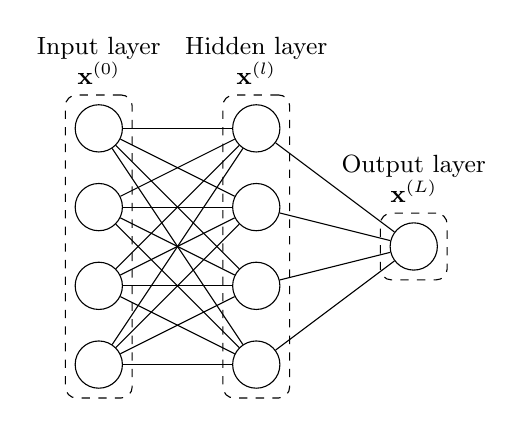
\begin{tikzpicture}

\tikzstyle{neuron}=[draw,circle,minimum width=0.6cm]
\tikzstyle{every node}=[font=\small]
\tikzstyle{every label}=[align=center,font=\small]

\foreach \x in {0, 1, 2, 3} {
  \node[neuron] (input\x) at (0, \x) {};
  \node[neuron] (hidden\x) at (2, \x) {};
}

\node[neuron] (output) at (4, 1.5) {};

\node[fit=(input0)(input3),draw,rounded corners=4pt, dashed,label=90:Input
layer\\$\vect{x}^{(0)}$] {};

\node[fit=(hidden0)(hidden3),draw,rounded corners=4pt, dashed,label=90:Hidden
layer\\$\vect{x}^{(l)}$] {};

\node[fit=(output),draw,rounded corners=4pt, dashed,label=90:Output
layer\\$\vect{x}^{(L)}$] {};

\foreach \x in {0, 1, 2, 3} {
  \foreach \y in {0, 1, 2, 3} {
    \draw (input\x)--(hidden\y);
  }
  \draw (hidden\x)--(output);
}
\end{tikzpicture}
\end{center}
\begin{block}{Activations of a layer of a neural network}
\vspace*{-1em}
\begin{align*}
x^{(l)}_j &= f\Big(\sum_i w^{(l)}_{ij}x^{(l-1)}_i\Big) & \text{for }l \in
[1,L]
\end{align*}
\end{block}
\end{frame}


% Instead of representing a vector of units, each layer represents a
% multichannel image, where each channel represents a 2D or 3D image


\begin{frame}{Convolutional Neural Network}
\begin{center}
\begin{tikzpicture}

\tikzstyle{neuron}=[draw,circle,minimum width=0.6cm]
\tikzstyle{every node}=[font=\small]
\tikzstyle{every label}=[align=center,font=\small]
\tikzstyle{every pin}=[align=center,font=\small,overlay]
\tikzstyle{every pin edge}=[overlay]

\foreach \x in {0, 1, 2, 3} {
  \ifnum\x=3
  \node<1-2>[neuron] (input\x) at (0, \x) {};
  \node<3->[neuron,pin=180:3D image] (input\x) at (0, \x) {};
  \else
  \node[neuron] (input\x) at (0, \x) {};
  \fi
  \node[neuron] (hidden\x) at (2, \x) {};
}

\node<3>[neuron,thick,red!80] at (0, 3) {};

\node[neuron,dashed] (output) at (4, 1.5) {};

\node<1>[fit=(input0)(input3),draw,rounded corners=4pt, dashed,label=90:Input
layer\\$x^{(0)}$] {};

\node<2>[fit=(input0)(input3),draw,rounded corners=4pt,label=90:Input
layer\\$x^{(0)}$,thick,red!80,pin=180:Multichannel\\image] {};

\node<3->[fit=(input0)(input3),draw,rounded corners=4pt,label=90:Input
layer\\$x^{(0)}$,dashed,pin=180:Multichannel\\image] {};

\node[fit=(hidden0)(hidden3),draw,rounded corners=4pt, dashed,label=90:Hidden
layer\\$x^{(l)}$] {};

% \node[fit=(output),draw,rounded corners=4pt, dashed,label=90:Output
% layer\\$x^{(L)}$] {};

\foreach \x in {0, 1, 2, 3} {
  \foreach \y in {0, 1, 2, 3} {
    \draw (input\x)--(hidden\y);
  }
  \draw[dashed] (hidden\x)--(output);
}

\only<4>{
  \draw[thick,red!80] (input3)--(hidden3);
}

\only<4->{
  \path (input3)--node[above,font=\small]{$*\tilde{w}^{(l)}_{ij}$} (hidden3);
}

% \only<5>{
%   \foreach \x in {0, 1, 2, 3} {
%     \draw[thick,red!80] (input\x)--(hidden3);
%   }
% }
% 
% \only<5->{
% \path (input3)--
%   node[above, align=center, font=\small]{Multichannel\\ filter kernel}
%   (hidden3);
% }

\end{tikzpicture}
\end{center}
\uncover<5>{
\begin{block}{Activations of a convolutional layer}
\vspace*{-1em}
\begin{align*}
x^{(l)}_j &= f\Big(\sum_i \tilde{w}^{(l)}_{ij}*x^{(l-1)}_i\Big) & \text{for }l
\in [1,L]
\end{align*}
\end{block}
}
\end{frame}
\end{comment}

\begin{frame}{Convolutional Encoder Network: Architecture}

\begin{tikzpicture}

\tikzstyle{layer}=[dashed,inner sep=0,draw,rounded corners=4pt]
\tikzstyle{every node}=[font=\small]
\tikzstyle{every label}+=[align=center,font=\small]
\tikzstyle{connect}=[-latex,shorten <=4pt,shorten >=4pt]

% Inputs

\node[xshift=0.5cm,yshift=-1cm] (pd)
{\includegraphics[width=1.3cm]{images/teaser/PDw}};
\node (t2)
{\includegraphics[width=1.3cm]{images/teaser/T2w}};

\node[fit=(t2)(pd),layer,label=90:Input layer] (inputs) {};

% Hiddens

\node[right=1.4cm of inputs,xshift=0.4cm,yshift=-1cm] (h3)
{\includegraphics[width=1.1cm]{images/teaser/hiddens_044_5x1}};

\node[right=1.4cm of inputs] (h2)
{\includegraphics[width=1.1cm]{images/teaser/hiddens_044_1x4}};

\node[right=1.4cm of inputs,xshift=-0.4cm,yshift=1cm] (h1)
{\includegraphics[width=1.1cm]{images/teaser/hiddens_044_1x3}};

\node[fit=(h1)(h3),layer,label=90:Hidden layer] (hiddens) {};

% Prob mask

\node[right=1cm of hiddens] (prob)
{\includegraphics[width=1.3cm]{images/teaser/segmentation_044_p}};

\node[fit=(prob),layer,label=90:Probabilistic\\ mask] (pmask) {};

% Connections

\draw[connect] (inputs)--node[above] {$*$} (hiddens);
\draw[connect] (hiddens)--node[above] {$\circledast$}(pmask);

% Output

\node[right=1cm of pmask] (seg)
{\includegraphics[width=1.3cm]{images/teaser/segmentation_044_t}};

\node[fit=(seg),layer,label=90:Final\\ Segmentation] (hmask) {};
\draw[connect] (pmask)--node[above]{$>t$}(hmask);

\draw[decorate,decoration={brace,mirror,raise=10pt}]
(inputs.west|-hiddens.south)--
node[below=12pt] {Convolutional layer}(hiddens.south east);

\draw[decorate,decoration={brace,mirror,raise=36pt}]
(hiddens.south west)--
node[below=38pt] {Deconvolutional layer} (hiddens.south-|pmask.east);

\end{tikzpicture}
\footlineextra{[Brosch et al., MICCAI 2015]}
\end{frame}

\begin{frame}{Convolutional Encoder Network: Training}

\begin{enumerate}
\item Initialize filters with random values
\item Calculate initial guess of the segmentation
\item Optimize filters using stochastic gradient descent
\end{enumerate}

\begin{tikzpicture}

\tikzstyle{layer}=[dashed,inner sep=0,draw,rounded corners=4pt]
\tikzstyle{every node}=[font=\small]
\tikzstyle{every label}+=[align=center,font=\small]
\tikzstyle{connect}=[-latex,shorten <=4pt,shorten >=4pt]
\tikzstyle{bconnect}=[latex-latex,shorten <=4pt,shorten >=4pt]

% Inputs
%1, 3, 5, 8, 10, 13, 18, 22, 26, 33, 40, 44
\only<1>{\def\number{001}}
\only<2>{\def\number{003}}
\only<3>{\def\number{005}}
\only<4>{\def\number{008}}
\only<5>{\def\number{010}}
\only<6>{\def\number{013}}
\only<7>{\def\number{018}}
\only<8>{\def\number{022}}
\only<9>{\def\number{026}}
\only<10>{\def\number{033}}
\only<11>{\def\number{040}}
\only<12>{\def\number{044}}

\node[xshift=0.5cm,yshift=-1cm] (pd)
{\includegraphics[width=1.3cm]{images/teaser/PDw}};
\node (t2)
{\includegraphics[width=1.3cm]{images/teaser/T2w}};

\node[fit=(t2)(pd),layer,label=90:Input layer $x^{(0)}$] (inputs) {};

% Hiddens

\node[right=1.4cm of inputs,xshift=0.4cm,yshift=-1cm] (h3)
{\includegraphics[width=1.1cm]{images/teaser/hiddens_\number_5x1}};

\node[right=1.4cm of inputs] (h2)
{\includegraphics[width=1.1cm]{images/teaser/hiddens_\number_1x4}};

\node[right=1.4cm of inputs,xshift=-0.4cm,yshift=1cm] (h1)
{\includegraphics[width=1.1cm]{images/teaser/hiddens_\number_1x3}};

\node[fit=(h1)(h3),layer,label=90:Hidden layer $x^{(1)}$] (hiddens) {};

% Prob mask

\node[right=1.2cm of hiddens,xshift=0.25cm,yshift=-0.5cm] (hard)
{\includegraphics[width=1.3cm]{images/teaser/segmentation_\number_p}};

\node[right=1.2cm of hiddens,xshift=-0.25cm,yshift=0.5cm] (prob)
{\includegraphics[width=1.3cm]{images/teaser/segmentation_\number_t}};

\node[fit=(prob)(hard),layer,label=90:Lesion masks $x^{(2)}$] (pmask)
{};

% Connections

\draw[connect] (inputs)--node[above] {$*$} (hiddens);
\draw[connect] (hiddens)--node[above] {$\circledast$}(pmask);

% Output

\node[right=1cm of pmask] (seg)
{\includegraphics[width=1.3cm]{images/teaser/groundtruth}};

\node[fit=(seg),layer,label=90:Target $y$] (hmask) {};
\draw[bconnect] (pmask)--node[above]{$\Delta$}(hmask);

\end{tikzpicture}

\end{frame}

% \begin{frame}[fragile]{Movie test}
% % \includemedia[
% %   activate=pageopen,
% %   width=5cm,height=3cm,
% %   addresource={segmentationp.mp4},
% %   flashvars={%
% %      source=segmentationp.mp4% same path as in addresource!
% % %   &autoPlay=true%    % optional configuration
% % %   &loop=true%        % variables
% %   }
% % ]{}{VPlayer.swf}
% 
% \includemedia[
%   activate=pageopen,
%   width=5cm,keepaspectratio,
%   addresource={segmentationp.mp4},
%   flashvars={source=segmentationp.mp4,autoPlay=true}
% ]{}{VPlayer.swf}
% \end{frame}

% \begin{frame}{Objective Function}
% \begin{itemize}
% \item Choice of an appropriate objective function important
% \item Sum of squared difference or cross-correlation
% \begin{itemize}
% \item $E = \frac{1}{2}\sum_{\vect{p}}\left(S(\vect{p}) -
% y^{(0)}(\vect{p})\right)^2$
% % , where $\vect{p} \in \N^3$ are the coordinates of a
% % particular voxel.
% \item Assigns same importance to every voxel
% \item Can learn to ignore the minority class 
% \item[$\Rightarrow$] Does not work well for unbalanced
% classes such as MS lesions
% \end{itemize}
% \item Combination of sensitivity and specificity
% \begin{itemize}
% \item Can be used together to measure segmentation performance
% \item Formulated as squared error terms to yield smooth gradients
% \item[$\Rightarrow$] Facilitates the segmentation of MS lesions 
% \end{itemize}
% \end{itemize}
% \end{frame}

\begin{frame}{Objective Functions}
%Choice of an appropriate objective function important
Sum of squared difference:
% \begin{equation*}
% E = \frac{1}{2}\sum_{\vect{p}}\left(S(\vect{p}) - y^{(0)}(\vect{p})\right)^2
% \end{equation*}
% % , where $\vect{p} \in \N^3$ are the coordinates of a
% % particular voxel.
\begin{itemize}
\item $\Delta = \frac{1}{2}\sum_{\vect{p}}\left(y(\vect{p}) -
x^{(2)}(\vect{p})\right)^2$
\item Assigns same importance to every voxel
\item Can learn to ignore the minority class% when both classes are very
%unbalanced
% \cons Does not work well for MS lesions
\end{itemize}
\vspace{0.5em}
Combination of \alert{sensitivity} and \alert{specificity}:
% \begin{multline*} 
% E = r\frac{\textstyle\sum_{\vect{p}} \left(S(\vect{p}) -
% y^{(0)}(\vect{p})\right)^2 S(\vect{p})}{\textstyle\sum_{\vect{p}} S(\vect{p})}
% 
%  + (1-r)\frac{\textstyle\sum_{\vect{p}} \left(S(\vect{p}) -
% y^{(0)}(\vect{p})\right)^2 \big(1 - S(\vect{p})\big)}{%
% \textstyle\sum_{\vect{p}}\big(1 - S(\vect{p})\big)}.
% \end{multline*}
\begin{itemize}
% \only<2>{
% \item $E = r\frac{\textstyle\sum_{\vect{p}}
% y^{(0)}(\vect{p})S(\vect{p})}{\textstyle\sum_{\vect{p}} S(\vect{p})}
%  + (1-r)\frac{\textstyle\sum_{\vect{p}} \left(1 -
% y^{(0)}(\vect{p})\right) \big(1 - S(\vect{p})\big)}{%
% \textstyle\sum_{\vect{p}}\big(1 - S(\vect{p})\big)}$}
\item $\Delta = r\frac{\textstyle\sum_{\vect{p}} \left(y(\vect{p}) -
x^{(2)}(\vect{p})\right)^2 y(\vect{p})}{\textstyle\sum_{\vect{p}}
y(\vect{p})}$\\
 \hspace{2cm}$+ (1-r)\frac{\textstyle\sum_{\vect{p}} \left(y(\vect{p}) -
x^{(2)}(\vect{p})\right)^2 \big(1 - y(\vect{p})\big)}{%
\textstyle\sum_{\vect{p}}\big(1 - y(\vect{p})\big)}$
\item Accuracies for both classes are calculated
separately and then combined to yield a single score
% \item Can be used together to measure segmentation performance
\item Formulated as squared error terms to yield smooth gradients
% \pros Facilitates the segmentation of MS lesions 
\end{itemize}
\footlineextra{[Brosch et al., MICCAI 2015]}
\end{frame}

\begin{comment}

\begin{frame}{Training in the Frequency Domain}
\begin{block}{Challenge}
Computational bottleneck is the calculation of 3D convolutions, which can
make training prohibitively slow.
\end{block}
\begin{itemize}
\item Perform training in the frequency domain
\item Replaces time-consuming convolutions with fast element-wise
multiplications
\item Minimize transitions between spatial and frequency domain by mapping
operations to frequency domain
\item Calculation of most time-consuming operations \alert{6 times faster} on
the GPU than the highly-optimized deep learning library provided by NVIDIA
\end{itemize}
% \small
% \begin{center}
% \begin{tabular}{ll}
% \toprule
% Operation in spatial domain & Operation in frequency domain\\
% \midrule
% Scalar multiplication & Scalar multiplication \\
% Element-wise addition & Element-wise addition \\
% Convolution & Element-wise multiplication \\
% Flipping of a kernel & Element-wise complex conjugate \\
% \bottomrule
% \end{tabular}
% \end{center}
\footlineextra{[Brosch and Tam, Neural Computation, 2015]}
\end{frame}
\end{comment}

\begin{frame}[fragile]{Network Architecture: 3-layer CEN}
\begin{columns}
\begin{column}{0.45\textwidth}
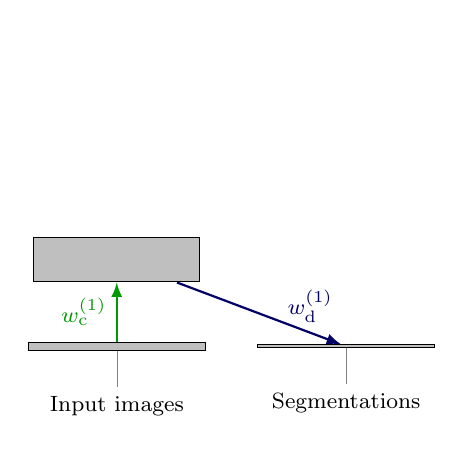
\begin{tikzpicture}[
  node distance=0.75cm and 0.65cm,
  font=\footnotesize,
  conv/.style={green!60!black,-latex,thick},
  conv2/.style={green!60!black,latex-latex,thick},
  deconv/.style={-latex,blue!40!black,thick},
  pooling/.style={-latex,green!60!black,thick,dashed},
  unpooling/.style={-latex,blue!40!black,thick,dashed},
  channel/.style args={#1 and #2}{draw, fill=lightgray, inner sep=0pt,
      minimum width=#1, minimum height=#2}
]

% Network

\node[channel=64pt and 3pt,pin=270:Input images] (inputs) {};
\node[channel=60pt and 16pt,above=of inputs] (clayer1) {};
\node[channel=64pt and 1pt,right=of inputs,pin=270:Segmentations] (outputs) {};

\begin{scope}[opacity=0]
\node[channel=30pt and 16pt,above=of clayer1] (pooling1) {};
\node[channel=60pt and 16pt] (dlayer1) at (clayer1-|outputs) {};
\node[channel=30pt and 16pt,above=of dlayer1] (dpooling1) {};
\node[fit=(pooling1)(dpooling1),inner sep = 0pt] (pooling) {};
\node[channel=26pt and 16pt,above=of pooling] (clayer2) {};
\end{scope}

\draw[conv] (inputs)--node[left] {$w^{(1)}_\text{c}$} (clayer1);
%\draw[pooling] (clayer1)--node[left] {} (pooling1);
%\draw[conv] (pooling1)--node[left] {$w^{(3)}_\text{c}$} (clayer2);
%\draw[deconv] (clayer2)--node[right=5pt] {$w^{(3)}_\text{d}$} (dpooling1);
%\draw[unpooling] (dpooling1)--node[right] {} (dlayer1);
%\draw[deconv] (dlayer1)--node[right] {$w^{(1)}_\text{d}$} (outputs);
\draw[deconv] (clayer1)--node[anchor=188,inner sep=10pt]
{$w^{(1)}_\text{d}$}(outputs);

\end{tikzpicture}
\end{column}
\begin{column}{0.55\textwidth}
\centering
\begin{tikzpicture}
\node[inner sep=0pt] (image) {
  \includegraphics[width=0.45\textwidth]{images/p50s35_large_lesions_a}
};
\draw[white,thick] (-11pt,-14pt) circle (8pt);
\draw[white,thick] (13pt,-14pt) circle (9pt);

\end{tikzpicture}%
\hspace{4pt}%
\begin{tikzpicture}
[spy using outlines={circle, magnification=4, connect spies}]

\node[inner sep=0pt] (image) {
  \includegraphics[width=0.45\textwidth]{images/p25s35_small_lesions_a}
};
\spy[white,thick, size=24pt,magnification=8] on (-9pt,18pt) in node[overlay]
at (-20pt,44pt);
\spy[white,thick, size=40pt] on (0pt,3pt) in node[overlay] at (24pt, 44pt);
\spy[white,thick, size=24pt, magnification=6] on (-11.5pt,-10.5pt) in
node[overlay] at (10pt,-46pt);

\node[below=1.5em of image,overlay,font=\footnotesize,align=right] {%
\textcolor{green!80!black}{Detected lesions}\\
\textcolor{yellow!80!black}{Missed lesions}\\
\textcolor{red!80!black}{False positives}};
\end{tikzpicture}
\end{column}
\end{columns}
\footlineextra{[Brosch et al., TMI 2016]}
\end{frame}

\begin{frame}[fragile]{Network Architecture: 7-layer CEN}
\begin{columns}
\begin{column}{0.45\textwidth}
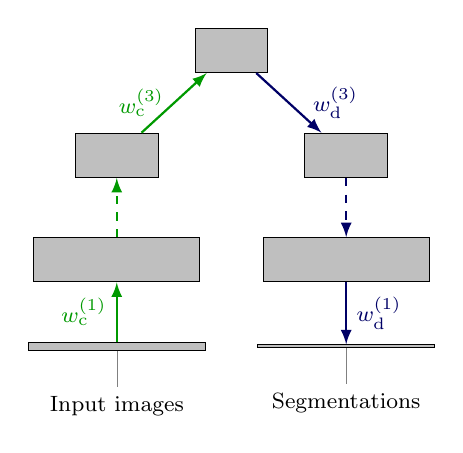
\begin{tikzpicture}[
  node distance=0.75cm and 0.65cm,
  font=\footnotesize,
  conv/.style={green!60!black,-latex,thick},
  conv2/.style={green!60!black,latex-latex,thick},
  deconv/.style={-latex,blue!40!black,thick},
  pooling/.style={-latex,green!60!black,thick,dashed},
  unpooling/.style={-latex,blue!40!black,thick,dashed},
  channel/.style args={#1 and #2}{draw, fill=lightgray, inner sep=0pt,
      minimum width=#1, minimum height=#2}
]

% Network

\node[channel=64pt and 3pt,pin=270:Input images] (inputs) {};
\node[channel=60pt and 16pt,above=of inputs] (clayer1) {};
\node[channel=30pt and 16pt,above=of clayer1] (pooling1) {};

\node[channel=64pt and 1pt,right=of inputs,pin=270:Segmentations] (outputs) {};
\node[channel=60pt and 16pt] (dlayer1) at (clayer1-|outputs) {};
\node[channel=30pt and 16pt,above=of dlayer1] (dpooling1) {};
\node[fit=(pooling1)(dpooling1),inner sep = 0pt] (pooling) {};
\node[channel=26pt and 16pt,above=of pooling] (clayer2) {};

\draw[conv] (inputs)--node[left] {$w^{(1)}_\text{c}$} (clayer1);
\draw[pooling] (clayer1)--node[left] {} (pooling1);
\draw[conv] (pooling1)--node[left] {$w^{(3)}_\text{c}$} (clayer2);
\draw[deconv] (clayer2)--node[right=5pt] {$w^{(3)}_\text{d}$} (dpooling1);
\draw[unpooling] (dpooling1)--node[right] {} (dlayer1);
\draw[deconv] (dlayer1)--node[right] {$w^{(1)}_\text{d}$} (outputs);
% \draw[deconv] (clayer1)--node[anchor=188,inner sep=10pt]
% {$w^{(1)}_\text{s}$}(outputs);

\end{tikzpicture}
\end{column}
\begin{column}{0.55\textwidth}
\centering
\begin{tikzpicture}
\node[inner sep=0pt] (image) {
  \includegraphics[width=0.45\textwidth]{images/p50s35_large_lesions_b}
};
\draw[white,thick] (-11pt,-14pt) circle (8pt);
\draw[white,thick] (13pt,-14pt) circle (9pt);

\end{tikzpicture}%
\hspace{4pt}%
\begin{tikzpicture}
[spy using outlines={circle, magnification=4, connect spies}]

\node[inner sep=0pt] (image) {
  \includegraphics[width=0.45\textwidth]{images/p25s35_small_lesions_b}
};
\spy[white,thick, size=24pt,magnification=8] on (-9pt,18pt) in node[overlay]
at (-20pt,44pt);
\spy[white,thick, size=40pt] on (0pt,3pt) in node[overlay] at (24pt, 44pt);
\spy[white,thick, size=24pt, magnification=6] on (-11.5pt,-10.5pt) in
node[overlay] at (10pt,-46pt);

\node[below=1.5em of image,overlay,font=\footnotesize,align=right] {%
\textcolor{green!80!black}{Detected lesions}\\
\textcolor{yellow!80!black}{Missed lesions}\\
\textcolor{red!80!black}{False positives}};
\end{tikzpicture}
\end{column}
\end{columns}
\footlineextra{[Brosch et al., TMI 2016]}
\end{frame}

\begin{frame}[fragile]{Network Architecture: 7-layer CEN with shortcut}
\begin{columns}
\begin{column}{0.45\textwidth}
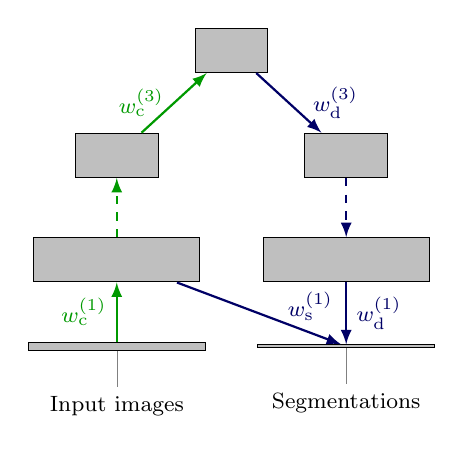
\begin{tikzpicture}[
  node distance=0.75cm and 0.65cm,
  font=\footnotesize,
  conv/.style={green!60!black,-latex,thick},
  conv2/.style={green!60!black,latex-latex,thick},
  deconv/.style={-latex,blue!40!black,thick},
  pooling/.style={-latex,green!60!black,thick,dashed},
  unpooling/.style={-latex,blue!40!black,thick,dashed},
  channel/.style args={#1 and #2}{draw, fill=lightgray, inner sep=0pt,
      minimum width=#1, minimum height=#2}
]

% Network

\node[channel=64pt and 3pt,pin=270:Input images] (inputs) {};
\node[channel=60pt and 16pt,above=of inputs] (clayer1) {};
\node[channel=30pt and 16pt,above=of clayer1] (pooling1) {};

\node[channel=64pt and 1pt,right=of inputs,pin=270:Segmentations] (outputs) {};
\node[channel=60pt and 16pt] (dlayer1) at (clayer1-|outputs) {};
\node[channel=30pt and 16pt,above=of dlayer1] (dpooling1) {};
\node[fit=(pooling1)(dpooling1),inner sep = 0pt] (pooling) {};
\node[channel=26pt and 16pt,above=of pooling] (clayer2) {};

\draw[conv] (inputs)--node[left] {$w^{(1)}_\text{c}$} (clayer1);
\draw[pooling] (clayer1)--node[left] {} (pooling1);
\draw[conv] (pooling1)--node[left] {$w^{(3)}_\text{c}$} (clayer2);
\draw[deconv] (clayer2)--node[right=5pt] {$w^{(3)}_\text{d}$} (dpooling1);
\draw[unpooling] (dpooling1)--node[right] {} (dlayer1);
\draw[deconv] (dlayer1)--node[right] {$w^{(1)}_\text{d}$} (outputs);
\draw[deconv] (clayer1)--node[anchor=188,inner sep=10pt]
{$w^{(1)}_\text{s}$}(outputs);

\end{tikzpicture}
\end{column}
\begin{column}{0.55\textwidth}
\centering
\begin{tikzpicture}
\node[inner sep=0pt] (image) {
  \includegraphics[width=0.45\textwidth]{images/p50s35_large_lesions_c}
};
\draw[white,thick] (-11pt,-14pt) circle (8pt);
\draw[white,thick] (13pt,-14pt) circle (9pt);

\end{tikzpicture}%
\hspace{4pt}%
\begin{tikzpicture}
[spy using outlines={circle, magnification=4, connect spies}]

\node[inner sep=0pt] (image) {
  \includegraphics[width=0.45\textwidth]{images/p25s35_small_lesions_c}
};
\spy[white,thick, size=24pt,magnification=8] on (-9pt,18pt) in node[overlay]
at (-20pt,44pt);
\spy[white,thick, size=40pt] on (0pt,3pt) in node[overlay] at (24pt, 44pt);
\spy[white,thick, size=24pt, magnification=6] on (-11.5pt,-10.5pt) in
node[overlay] at (10pt,-46pt);

\node[below=1.5em of image,overlay,font=\footnotesize,align=right] {%
\textcolor{green!80!black}{Detected lesions}\\
\textcolor{yellow!80!black}{Missed lesions}\\
\textcolor{red!80!black}{False positives}};

\end{tikzpicture}
\end{column}
\end{columns}
\footlineextra{[Brosch et al., TMI 2016]}
\end{frame}

\subsection{Evaluation}

\begin{frame}{Evaluation}
Evaluated on two data sets:
\begin{itemize}
\item MICCAI 2008 MS Lesion Segmentation Challenge
\begin{itemize}
\item 20 training, 23 testing images
\item Modalities: T1w, T2w, FLAIR 
\end{itemize}
\item Clinical trial data set
\begin{itemize}
\item 250 training, 77 testing images
\item Modalities: T1w, T2w, PDw, FLAIR
\item Compared to 5 freely available methods
\item Stratified by average lesion size
\end{itemize}
\end{itemize}
\vspace{0.5em}
Evaluation measures:
\begin{itemize}
\item Dice similarity coefficient (DSC)
\item Lesion true positive rate (LTPR)
\item Lesion false positive rate (LFPR)
\item Volume difference (VD)
\end{itemize}
\end{frame}

% Mention that the score is a compound score

\begin{frame}{MICCAI 2008 Lesion Segmentation Challenge}
\small
\sisetup{
  round-mode = places,
  round-precision = 2,
  detect-weight=true}%
Selected methods out of the 52 entries submitted for evaluation to the
MICCAI 2008 MS lesion segmentation challenge.
\begin{center}
\begin{tabular}{@{}clS[table-format=2.2]
S[table-format=2.1,round-precision=1]
S[table-format=2.1,round-precision=1]
S[table-format=2.1,round-precision=1]@{}}
\toprule
Rank & Method & {Score} & {LTPR} & {LFPR} & {VD} \\
\midrule
$1,3,9$  & Jesson et al. (2015) & 86.9386 & 48.70 & 28.25 & 80.15 \\
2  & Guizard et al. (2015)  & 86.1071 & 49.85 & 42.75 & 48.80 \\
$4,20,26$  & Tomas-Fernandez et al. (2012) & 84.464 & 46.9 & 44.6 &
45.60 \\
$5,7$ & Jerman et al. (2015) & 84.1555 & 65.15 & 63.75 & 77.45 \\
\bfseries 6  & \bfseries Our method  & \bfseries 84.0743 & \bfseries
51.55 & \bfseries 51.25 & \bfseries 57.75 \\
11 & Roura et al. (2015)   & 82.3442 & 50.15 & 41.85 & 111.60 \\
13 & Geremia et al. (2010) & 82.0691 & 55.1 & 74.1 & 48.90 \\
24 & Shiee et al. (2010) & 79.8975 & 52.4 & 72.7 & 74.45 \\
33 & Sudre et al. (2014) & 77.9601 & 22.3 & 18.1 & 285.6 \\
\bottomrule
\end{tabular}
\end{center}
\footlineextra{[Brosch et al., TMI 2016]}
\end{frame}

\begin{frame}{Clinical Trial Data Set}
\vspace{2em}
\begin{center}
\tikz[overlay] \node{%
\includegraphics[width=\textwidth]{images/dsc_arch}};
\end{center}
\footlineextra{[Brosch et al., TMI 2016]}
\end{frame}

\begin{frame}{Clinical Trial Data Set}
\vspace{2em}
\begin{center}
\tikz[overlay] \node{%
\includegraphics[width=1.1\textwidth]{images/dsc_meth}};
\end{center}
\footlineextra{[Brosch et al., TMI 2016]}
\end{frame}

% \begin{frame}{Stratified by Lesion Size: Lesion TPR}
% \begin{center}
% \tikz[overlay] \node{%
% \includegraphics[width=1.1\textwidth]{images/ltpr_def}};
% \end{center}
% \end{frame}
% 
% \begin{frame}{Stratified by Lesion Size: Lesion FPR}
% \begin{center}
% \tikz[overlay] \node{%
% \includegraphics[width=1.1\textwidth]{images/lfpr_def}};
% \end{center}
% \end{frame}

\section{Manifold Learning}

\subsection{Manifold Learning of Brain MRIs}

\begin{frame}{Manifold Learning}
\tikz\node[inner sep=0,align=left,opacity=0.2,text width=0.99\textwidth] {%
\begin{itemize}
\item Developed a computation and memory efficient training algorithm for
convolutional deep learning models
\item Developed a novel segmentation method that learns features at
different scales that are tuned to a given combination of image types and
segmentation task
\item Proposed a novel objective function that facilitates the training using
vastly unbalanced training sets, such as is the case for segmenting MS lesions
\end{itemize}};
\begin{itemize}
\item First work to demonstrate the use of deep learning for manifold learning
of 3D medical images
\item Developed a framework for modelling changes in brain morphology and lesion
distribution
\end{itemize}
\end{frame}

% \begin{frame}{Manifold Learning}
% 
% \begin{block}{Objective}
% To model the variability of brain images affected by Alzheimer's disease and
% multiple sclerosis in order to derive new imaging biomarkers.
% \end{block}
% 
% \begin{block}{Manifold assumption}
% The intrinsic dimensionality of the data is much lower than the number of
% dimensions of a data point. Hence, the data lies in a low-dimensional manifold
% embedded in the high-dimensional ambient space.
% \end{block}
% 
% Manifold learning:
% \begin{itemize}
% \item To discover the low-dimensional manifold space
% \item Manifold coordinates correspond to the modes of variation
% \item Manifolds can be highly nonlinear
% \end{itemize}
% 
% %\footlineextra{[Brosch and Tam, MICCAI 2013; Brosch et al., MICCAI 2014]}
% \end{frame}

\begin{frame}{Modelling Variability by Manifold Learning}

\begin{block}{Toy Example: Rotated Brain MRIs}
\begin{center}
\begin{tikzpicture}
\node {\includegraphics[width=1.8cm]{images/mediumatrophy}};
\node at (2,0) {\includegraphics[width=1.8cm]{images/mediumatrophy_r1}};
\node at (4,0) {\includegraphics[width=1.8cm]{images/mediumatrophy_r2}};
\node at (6,0) {\includegraphics[width=1.8cm]{images/mediumatrophy_r3}};
\end{tikzpicture}
\end{center}
\end{block}
% \begin{block}{Manifold assumption}
% Brain images lie on a low-dimensional manifold, where the manifold coordinates
% represent the modes of variation of the data.
% \end{block}
\begin{itemize}
\item \alert{Manifold assumption:} Brain images lie on a low-dimensional
manifold, where the manifold coordinates represent the modes of variation.
%\item Data dimensions: Voxel intensities
%\item Manifold dimensions: Modes of variation (e.g., rotations)
\item[\faQuestionCircle] What are the modes of variations of brain images
affected by Alzheimer's disease and multiple sclerosis?
\item[\faQuestionCircle] Can the manifold coordinates be used to measure disease
state and progression?
\end{itemize}
\end{frame}

% Stacking multiple RBMs to discover increasingly abstract and nonlinear
% patterns

\begin{frame}{Manifold Learning of Brain MRIs by Deep Learning}
% Related Work:
% \begin{itemize}
% \item Global methods (e.g., Isomap)
% \item Local methods (e.g., locally linear embedding)
% \cons Require the definition of a similarity measure and a neighborhood
% criteria
% \end{itemize}
% \vspace{0.5em}
Proposed Framework:
\begin{itemize}
% \item Manifold learning performed using a stack of restricted Boltzmann machines
% (RBMs)
% \item Each RBM reduces the dimensionality of its inputs by discovering patterns
% of similarity
\item Based on deep belief networks
\item Fewer assumptions than alternative manifold learning methods
\end{itemize}
\begin{center}

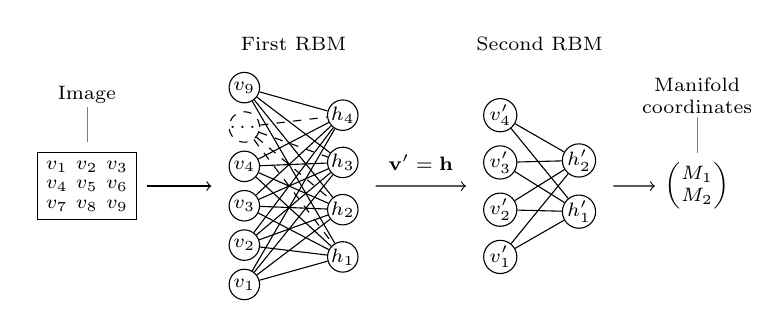
\begin{tikzpicture}
  \tikzstyle{every node}+=[font=\scriptsize]
  \tikzstyle{gnode}=[shape=circle,draw=black,inner sep=0pt,
  minimum width=11pt] 
  \tikzstyle{featuremap}=[draw,fill=white,fill opacity=1,
matrix of math nodes, inner sep=1.5pt]
\tikzstyle{every pin}+=[inner sep=1pt,align=center]
  
  % Image
  \matrix[featuremap] (image) {
    v_1 & v_2 & v_3 \\
    v_4 & v_5 & v_6 \\
    v_7 & v_8 & v_9 \\
  };
  
  \node[fit=(image),pin=90:Image] (bimage) {};
  
  % RBM 1
  
  \foreach \x in {1,...,6} {
  \ifnum\x=5
    \node[gnode,dashed] (v\x) at (2, 0.5*\x - 1.75) {\scriptsize\ldots};
  \else
  \ifnum\x=6
    \node[gnode] (v\x) at (2, 0.5*\x - 1.75) {$v_9$};
  \else
    \node[gnode] (v\x) at (2, 0.5*\x - 1.75) {$v_\x$};
  \fi
  \fi
  }
  
  \foreach \y in {1,...,4} {
    \node[gnode] (h\y) at (3.25, 0.6*\y - 1.5) {$h_\y$};
  }

  \foreach \x in {1,...,6} {
    \foreach \y in {1,...,4} {
      \ifnum\x=5
        \draw[dashed] (v\x)--(h\y);
      \else
        \draw (v\x)--(h\y);
      \fi
    }
  }
  
  \node[fit=(v1)(v6)(h1),inner sep=6pt,overlay] (brbm1) {};
  
  % RBM 2
  
  \tikzstyle{gnode}=[shape=circle,draw=black,inner sep=0pt,
  minimum width=12pt] 
  
  \foreach \x in {1,...,4} {
    \node[gnode] (v\x) at (5.25, 0.6*\x - 1.5) {$v'_\x$};
  }
  
  \foreach \y in {1,...,2} {
    \node[gnode] (h\y) at (6.25, 0.65*\y - 0.975) {$h'_\y$};
  }

  \foreach \x in {1,...,4} {
    \foreach \y in {1,...,2} {
        \draw (v\x)--(h\y);
    }
  }
  
  \node[fit=(v1)(v4)(h1),inner sep=6pt,overlay] (brbm2) {};
  
  % Manifold coordinates
  
  \node[pin=90:Manifold\\ coordinates] (coordinates) at (7.75, 0) {
  $\begin{pmatrix}M_1 \\ M_2\end{pmatrix}$
  };
  
  % Annotations
  
  \draw[->] (bimage)--(brbm1);
  \draw[->] (brbm1)--node[above=2pt] {$\vect{v}' = \vect{h}$} (brbm2);
  \draw[->] (brbm2)--(coordinates);
  
  \coordinate (annotations) at ($(brbm1.north) + (0,4pt)$);
  
  \node at (annotations-|brbm1) {First RBM};
  \node at (annotations-|brbm2) {Second RBM};
  
  \end{tikzpicture}
  %}

\end{center}
\footlineextra{[Brosch and Tam, MICCAI 2013]}
\end{frame}

\begin{frame}{Manifold Learning of Brain MRIs by Deep Learning}
\begin{center}
\input{tikzfigures/manifold_dbn}
\end{center}
\footlineextra{[Brosch and Tam, MICCAI 2013]}
\end{frame}

% Results

% \begin{frame}{Manifold of Brain MRIs}
% \begin{itemize}
% \item Use a strided convolutional deep belief network
% \item Generative probabilistic model consisting of multiple layers of RBMs
% \item RBMs reduces the dimensionality of the data by discovering patterns of
% similarity
% \item Visible units input, hiddens are the patterns
% \item Through the stacking of multiple RBMs, a DBN can learn increasingly more
% nonlinear patterns.
% \end{itemize}
% \end{frame}

% Mention first use of deep learning for manifold learning of 3D medical images

\begin{frame}{Evaluation}
Data set:
\begin{itemize}
\item 300 T1-weighted MRIs of AD (150) and normal (150) subjects from the ADNI
data set
\item Number of voxels: \num{128x128x128}
\item Voxel size: \SI{2x2x2}{\milli\metre}
\end{itemize}

Experiments:
\begin{itemize}
\item Visualization of patterns of variability
\item Visualization of population differences in manifold space
\end{itemize}
\footlineextra{[Brosch and Tam, MICCAI 2013]}
\end{frame}

\begin{frame}{Visualizing the Modes of Variation}
\begin{columns}
\begin{column}{0.5\textwidth}
\begin{tikzpicture}
\tikzstyle{every node}+=[font=\small]
\node[inner sep=6pt] (manifold)
{\includegraphics[width=0.9\textwidth]{images/MICCAI2013_sampled2d}};

\draw[->,overlay] (manifold.south west)--node[below=5pt,inner sep=0] {$M_1$}
(manifold.south east);
\draw[->] (manifold.south west)--node[above=5pt,sloped,inner sep=0]
{$M_2$} (manifold.north west);

\end{tikzpicture}
\end{column}
\begin{column}{0.5\textwidth}
\begin{itemize}
\item $M_1$ visually correlates with an increase in brain size
\item $M_2$ visually correlates with an increase in ventricle size
\end{itemize}
\end{column}
\end{columns}
\footlineextra{[Brosch and Tam, MICCAI 2013]}
\end{frame}

\begin{frame}{Visualization of the Data Set in Manifold Space}
\centering
\includegraphics[width=\textwidth]{images/scatterimage}
\footlineextra{[Brosch and Tam, MICCAI 2013]}
\end{frame}

\subsection{Modelling the Variability of MS Brains}

\begin{frame}{Modelling the Variability of MS Brains}
\begin{itemize}
\item[\faQuestionCircle] What are the predominant morphological variations in
MS?
\item[\faQuestionCircle] How are MS lesions distributed?
\item[\faQuestionCircle] How do these key pathological features interact?
\item Enforce the learning of morphological and lesion distribution
changes
\item DBN trained on \alert{deformation fields} and binary \alert{lesion masks}
\end{itemize}
\footlineextra{[Brosch et al, MICCAI 2014]}
\end{frame}

\begin{frame}{Model}
\centering
\hspace*{-1em}
\input{tikzfigures/jointmodel}
\footlineextra{[Brosch et al, MICCAI 2014]}
\end{frame}

\begin{frame}{Evaluation}
Data set:
\begin{itemize}
\item 474 T1-weighted, T2-weighted, and PD-weighted MRIs of secondary
progressive MS patients
\item Number of voxels: \num{256x256x50}
\item Voxel size: \SI{0.937x0.937x3.00}{\milli\metre}
\end{itemize}
Experiments:
\begin{itemize}
\item Visualization of patterns of morphological and lesion distribution changes
\item Correlation of manifold coordinates with MS clinical scores
\end{itemize}
\footlineextra{[Brosch et al, MICCAI 2014]}
\end{frame}

\begin{frame}{Morphology and Lesion Distribution Patterns}
\newlength{\subfigwidth}
\setlength{\subfigwidth}{0.35\textwidth}
\centering
\begin{tikzpicture}
\tikzstyle{every node}+=[font=\small]
\node
(manifold){\includegraphics[width=\subfigwidth]{images/MICCAI2014_warps_t1_dark}};

\draw[->] (manifold.south west)--node[below=5pt,inner sep=0] {$D_1$}
(manifold.south east);
\draw[->] (manifold.south west)--node[above=5pt,sloped,inner sep=0] {$D_2$}
(manifold.north west);

\end{tikzpicture}
\quad
\begin{tikzpicture}
\tikzstyle{every node}+=[font=\small]
\node
(manifold){\includegraphics[width=\subfigwidth]{images/MICCAI2014_viridis_p442_d0_full_h16-2}};

\draw[->] (manifold.south west)--node[below=5pt,inner sep=0] {$L_1$}
(manifold.south east);
\draw[->] (manifold.south west)--node[above=5pt,sloped,inner sep=0] {$L_2$}
(manifold.north west);

\node[inner sep=0, draw, rotate=90] at ([xshift=14pt]manifold.east) (colormap)
{\includegraphics[width=\subfigwidth,height=0.25cm]{images/viridis_scale}};

\node[below] at (colormap.west) {low};
\node[above] at (colormap.east) {high};

\end{tikzpicture}
\footlineextra{[Brosch et al, MICCAI 2014]}
\end{frame}

\begin{frame}{Joint Patterns of Variability}
\centering
\setlength{\subfigwidth}{0.48\textwidth}
\begin{tikzpicture}
\tikzstyle{every node}+=[font=\small]

\node[align=left,fill=black,inner sep = 0pt] (manifold1) {
  \mbox{}\\[2pt]
  \includegraphics[trim=0 340 0 0,clip,width=\subfigwidth]
    {images/MICCAI2014_viridis_full_rl1_h4_sag}\\[8.5pt]
  \includegraphics[trim=0 0 0 150,clip,width=\subfigwidth]
    {images/MICCAI2014_viridis_full_rl1_h4}
};
\node[fit=(manifold1)] (manifold) { };

\foreach \x/\y in {0.125/1, 0.375/2, 0.625/3, 0.875/4} {
  \node[left=1pt,inner sep=0pt] at ($(manifold.north west)!\x!(manifold.south
  west)$) {$J_\y$}; }

\draw[->] (manifold.south west)--node[below=5pt,inner sep=0] {$J_x$}
(manifold.south east);

\node[inner sep=0, draw, rotate=90] at ([xshift=14pt]manifold.east) (colormap)
{\includegraphics[width=\subfigwidth,height=0.25cm]{images/viridis_scale}};

\node[below] at (colormap.west) {low};
\node[above] at (colormap.east) {high};

\end{tikzpicture}
\footlineextra{[Brosch et al, MICCAI 2014]}
\end{frame}

% Mention: better correlations

\begin{frame}{Pearson Correlations with Clinical Scores}
\footnotesize

% Comparison of correlations of manifold coordinates and imaging biomarkers
% (normalized brain volume, nBV; lesion load, LL) with clinical scores (timed 25
% feet walk, T25W; 9-hole peg test, 9-HPT; paced auditory sequential addition
% test, PASAT; MS functional composite, MSFC):

\sisetup{
  round-mode = places,
  round-precision = 3,
  exponent-product = \cdot,
  detect-weight=true,
  detect-inline-weight=math,
  tight-spacing = false,
  table-align-text-post = false
}%

\def\tabspace{14pt}

\begin{tabular}{@{}c@{\hspace{\tabspace}}c%
@{\hspace{\tabspace}}S[table-format=2.5]%
@{\hspace{\tabspace}}S[table-format=2.6]
@{\hspace{\tabspace}}S[table-format=2.6]
@{\hspace{\tabspace}}S[table-format=2.6]@{}}
\toprule
 &  & {T25W} & {9-HPT} & {PASAT} & {MSFC} \\
 \midrule
 
\multirow{4}*{\minitab[c]{Individual\\ models}}
 & $D_1$ &
\bfseries -0.128976787246536** & -0.214588136146619*** & -0.282044527648157*** &
-0.314633263656368*** \\
 & $D_2$ & 0.0870255979372807 & 0.115835195120173* & 0.08923208653141 &
0.138616500875685** \\
& $L_1$ & -0.0581629511079419 & -0.231012897586838*** & -0.391822792658197*** &
-0.366992537420278*** \\
& $L_2$ & -0.091057480388512 & \bfseries -0.354478789398171*** &
\bfseries -0.426543205964196*** & \bfseries -0.463860459137063*** \\
\addlinespace
\multirow{4}*{\minitab[c]{Joint\\ model}}
 & $J_1$ & 0.107219513748914* & 0.285812780188632*** & 0.336253511146623*** &
0.378889115681159*** \\
 & $J_2$ & -0.037731447660239 & -0.209982769437628*** & -0.226800472678912***
& -0.255585426983655*** \\
& $J_3$ & \bfseries -0.117780586822506* & \bfseries -0.369169927947271*** &
\bfseries -0.452556545437486*** & \bfseries -0.494130959187706*** \\
& $J_4$ & -0.0491209563011896 & -0.205764640863705*** & -0.382954826511733*** &
-0.345529171963859*** \\
\addlinespace
\multirow{2}*{\minitab[c]{Imaging\\ biomarkers}}
 & nBV & 0.0530068558456253 & 0.143905618421747** & 0.246833144651129***
& 0.234774254053599*** \\
 & LL & -0.073681606595365 & \bfseries -0.286360084620956*** &
\bfseries -0.399646128024074*** & \bfseries -0.406222020153583*** \\
  
 \bottomrule
\end{tabular}
\\[0.66em]
Abbreviations: Timed 25-Foot Walk (T25W), 9-Hole Peg Test (9-HPT), Paced
Auditory Serial Addition Test (PASAT), MS Functional Composite (MSFC), normalized brain volume
(nBV), lesion load (LL)\\[0.33em]
Significance levels: *$p < 0.05$, **$p < 0.01$, ***$p<0.001$
\end{frame}

% \begin{frame}{Visualizing the Progression of Secondary Progressive MS}
% \end{frame}

\section{Conclusions}

\subsection*{Summary and Contributions}

\begin{frame}{Summary and Conclusions} % What have I done
\begin{itemize}
\item Presented a novel training algorithm for convolutional models that
performs training in the frequency domain
\item Minimizes the number of FFTs through the mapping of operations to
the frequency domain
\item Significantly faster than the state-of-the-art spatial domain
implementation
\item Facilitates the application of convolutional deep learning models for 3D
neurological images analysis
\end{itemize}
\end{frame}

\begin{frame}{Summary and Conclusions} % What have I learned/implications
\begin{itemize}
\item Presented a fully automatic MS lesion segmentation method based on
convolutional encoder networks
\item Joint training of feature extraction and classification layers allows for
the learning of features that are tuned to any given combination of image types
and segmentation task
\item Our framework is very flexible and can be readily applied to various
segmentation problems
\vspace{0.5em}
\item Presented a novel method for the automatic discovery of patterns of
variability in multiple sclerosis
\item Framework allows for the visualization and quantification of morphology
and lesion distribution patterns
\item Parameters of our model correlate stronger with MS clinical scores than
volumetric imaging biomarkers
\end{itemize}
\end{frame}

\begin{frame}{Publications Arising from this Thesis}
\begin{itemize}
\item Brosch, Tom and R. Tam, for the ADNI. Manifold learning of brain MRIs
by deep learning. In: K. Mori et als. (Eds.): MICCAI 2013, Part II, LNCS 8150,
pages 633--640, 2013.
\item Brosch, Tom, Y. Yoo, A. Traboulsee, D.K.B. Li, and R. Tam. Modeling the
variability in brain morphology and lesion distribution in multiple sclerosis by
deep learning. In: P. Golland et al. (Eds.): MICCAI 2014, Part II, LNCS 8674,
pages 462--469, 2014.
\item Brosch, Tom and R. Tam. Efficient training of convolutional deep
belief networks in the frequency domain for application to high-resolution 2D
and 3D images. Neural Computation, 27(1), pages 211--227, 2015.
\end{itemize}
\end{frame}

\begin{frame}{Publications Arising from this Thesis}
\begin{itemize}
\item Brosch, Tom, Y. Yoo, L.Y.W. Tang, D.K.B. Li, A. Traboulsee, and R. Tam.
Deep convolutional encoder networks for multiple sclerosis lesion segmentation.
In: N. Navab et al. (Eds.): MICCAI 2015, Part III, LNCS 9351, pages 3--11, 2015.
\item Brosch, Tom, L.Y.W. Tang, Y. Yoo, D.K.B. Li, A. Traboulsee, and R. Tam.
Deep 3D convolutional encoder networks with shortcuts for multiscale feature
integration applied to multiple sclerosis lesion segmentation. IEEE Transactions
on Medical Imaging, 2016. \emph{(accepted)}
\end{itemize}
\end{frame}

\begin{questionmarks}
\begin{frame}
\centering
\large Thank you for your attention.
% Do you have any questions?
\end{frame}
\end{questionmarks}

\begin{comment}
\begin{frame}{Training of Convolutional Neural Networks}
\begin{center}
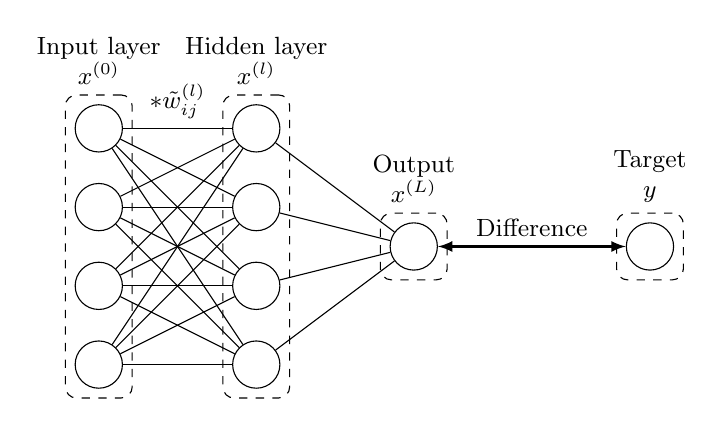
\begin{tikzpicture}

\tikzstyle{neuron}=[draw,circle,minimum width=0.6cm]
\tikzstyle{every node}=[font=\small]
\tikzstyle{every label}=[align=center,font=\small]
\tikzstyle{every pin}=[align=center,font=\small,overlay]
\tikzstyle{every pin edge}=[overlay]

\foreach \x in {0, 1, 2, 3} {
  \node[neuron] (input\x) at (0, \x) {};
  \node[neuron] (hidden\x) at (2, \x) {};
}

\node[neuron] (output) at (4, 1.5) {};

\node[neuron] (target) at (7, 1.5) {};

\node[fit=(input0)(input3),draw,rounded corners=4pt,label=90:Input
layer\\$x^{(0)}$,dashed] {};

\node[fit=(hidden0)(hidden3),draw,rounded corners=4pt, dashed,label=90:Hidden
layer\\$x^{(l)}$] {};

\node[fit=(output),draw,rounded corners=4pt, dashed,label=90:Output\\$x^{(L)}$] {};
\node[fit=(target),draw,rounded corners=4pt, dashed,label=90:Target\\$y$] {};

\only<2> {
\draw[latex-latex,thick] (output)--node[above,font=\small] {Difference}
  (target);
}

\foreach \x in {0, 1, 2, 3} {
  \foreach \y in {0, 1, 2, 3} {
    \draw (input\x)--(hidden\y);
  }
  \draw (hidden\x)--(output);
}

\path (input3)--node[above,font=\small]{$*\tilde{w}^{(l)}_{ij}$} (hidden3);

\end{tikzpicture}
\end{center}
\uncover<2>{
\begin{block}{Training objective}
To find the filter kernels such that the difference between the predicted output
and the expected output is minimized.
\end{block}
}
\end{frame}

\begin{frame}{Training of Convolutional Neural Networks}
\begin{center}
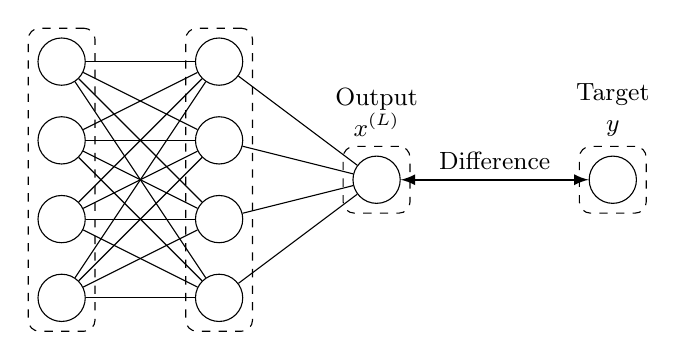
\begin{tikzpicture}

\tikzstyle{neuron}=[draw,circle,minimum width=0.6cm]
\tikzstyle{every node}=[font=\small]
\tikzstyle{every label}=[align=center,font=\small]
\tikzstyle{every pin}=[align=center,font=\small,overlay]
\tikzstyle{every pin edge}=[overlay]

\foreach \x in {0, 1, 2, 3} {
  \node[neuron] (input\x) at (0, \x) {};
  \node[neuron] (hidden\x) at (2, \x) {};
}

\node[neuron] (output) at (4, 1.5) {};
\node[neuron] (target) at (7, 1.5) {};

\node[fit=(input0)(input3),draw,rounded corners=4pt,dashed] {};
\node[fit=(hidden0)(hidden3),draw,rounded corners=4pt, dashed] {};
\node[fit=(output),draw,rounded corners=4pt, dashed,label=90:Output\\$x^{(L)}$] {};
\node[fit=(target),draw,rounded corners=4pt, dashed,label=90:Target\\$y$] {};

\draw[latex-latex,thick] (output)--node[above,font=\small] {Difference}
  (target);

\foreach \x in {0, 1, 2, 3} {
  \foreach \y in {0, 1, 2, 3} {
    \draw (input\x)--(hidden\y);
  }
  \draw (hidden\x)--(output);
}

\end{tikzpicture}
\end{center}
\begin{enumerate}
\item Forward pass: $x^{(l)}_j = f\Big(\sum_i\tilde{w}^{(l)}_{ij}*x^{(l-1)}_i\Big)$
\item Calculate $\delta^{(L)}$: $\delta^{(L)}_j = \big(x^{(L)}_j
-y_i\big)f'$
\item Calculate parameter update: $\Delta w^{(l)}_{ij} = x^{(l-1)}_i *
\tilde{\delta}^{(l)}_j$
\item Backpropagation: $\delta^{(l)}_i =
\sum_j^F\big(w^{(l+1)}_{ij}\circledast\delta^{(l+1)}_j\big)f'$
%\big(w^{(l+1)}_{ij}\circledast\delta^{(l+1)}_j\big)\I\big(x^{(l)}_i> 0\big)$
%\item Repeat from step 3 until the first layer is reached
\end{enumerate}
\end{frame}

\begin{frame}{Training in the Frequency Domain /1}
\tikzstyle{na} = [baseline=-.5ex,remember picture]
\small
\begin{columns}[t]
\begin{column}{0.7\textwidth}
Spatial domain
\begin{algorithm}[H]
\setstretch{1.15}
Initialize\;
\ForEach{image $\vect{v} \in \data$} {
  \tcp{Forward pass}
  \ForEach{filter $j$} {
    $x_j = 0$\;
    \ForEach{channel $i$} {
      $x_j = x_j + \tilde{w}_{ij} * x_i$\;
    }
  }
  \tcp{Backward pass}
  \ForEach{channel $i$} {
    $\delta_i = 0$\;
    \ForEach{filter $j$} {
      $\delta_i = \delta_i + w_{ij} \circledast \delta_j$\;
    }
  }
}
\end{algorithm}
\end{column}
\begin{column}{0.3\textwidth}
Frequency domain
\end{column}
\end{columns}
\end{frame}

\begin{frame}{Training in the Frequency Domain /2}
\tikzstyle{na} = [baseline=-.5ex,remember picture]
\small
\begin{columns}[t]
\begin{column}{0.7\textwidth}
\emph{Spatial domain}
\begin{algorithm}[H]
\setstretch{1.15}
Initialize\;
\ForEach{image $\vect{v} \in \data$} {
  \tcp{Forward pass\tikz[na] \coordinate (forward) at (1,0);}
  \ForEach{filter $j$} {
    $x_j = 0$\;
    \ForEach{channel $i$} {
      $x_j = x_j + z$\tikz[na] \coordinate (first) at (1,0);\;
    }
  }
  \tcp{Backward pass}
  \ForEach{channel $i$} {
    $\delta_i = 0$\;
    \ForEach{filter $j$} {
      $\delta_i = \delta_i + z$\tikz[na] \coordinate (second) at (1,0);\;
    }
  }
}
\end{algorithm}
\end{column}
\begin{column}{0.3\textwidth}
\emph{Frequency domain}\\
\begin{tikzpicture}[overlay,remember picture]

\coordinate (left);

% Forward
\draw[->, shorten >=10pt, shorten <=10pt] (forward) --
  node[above]{$\hat{x}=\mathcal{F}(x)$}
  (forward-|left);

\draw[->, shorten >=10pt, shorten <=10pt] ([yshift=2pt]first) --
  node[above]{$\hat{w}=\mathcal{F}(\tilde{w})$}
  ([yshift=2pt]first-|left);

\draw[<-, shorten >=10pt, shorten <=10pt] ([yshift=-2pt]first) --
  node[below]{$z = \mathcal{F}^{-1}(\hat{z})$}
  ([yshift=-2pt]first-|left);

\node[right] at (left|-first) {$\hat{z} = \hat{w} \cdot \hat{x}$};

% Backward
\draw[->, shorten >=10pt, shorten <=10pt] ([yshift=2pt]second) --
  node[above]{$\hat{\delta}=\mathcal{F}(\delta), \hat{w}=\mathcal{F}(w)$}
  ([yshift=2pt]second-|left);

\draw[<-, shorten >=10pt, shorten <=10pt] ([yshift=-2pt]second) --
  node[below]{$z = \mathcal{F}^{-1}(\hat{z})$}
  ([yshift=-2pt]second-|left);

\node[right] at (left|-second) {$\hat{z} = \hat{w}_{ij} \cdot \hat{\delta}_j$};

\end{tikzpicture}
\end{column}
\end{columns}
\end{frame}

\begin{frame}{Training in the Frequency Domain /3}
\tikzstyle{na} = [baseline=-.5ex,remember picture]
\small
\begin{columns}[t]
\begin{column}{0.7\textwidth}
\emph{Spatial domain}
\begin{algorithm}[H]
\setstretch{1.15}
Initialize\;
\ForEach{image $\vect{v} \in \data$} {
  \tcp{Forward pass}
  \ForEach{filter $j$} {
    $x_j = 0$\tikz[na] \coordinate (initx) at (1,0);\;
    $x_j = z$\tikz[na] \coordinate (writex) at (1,0);\;
    %\ForEach{channel $i$} {
    %  $x_j = x_j + z$\tikz[na] \coordinate (first) at (1,0);\;
    %}
  }
  \tcp{Backward pass}
  \ForEach{channel $i$} {
    $\delta_i = 0$\;
    \ForEach{filter $j$} {
      $\delta_i = \delta_i + z$\tikz[na] \coordinate (second) at (1,0);\;
    }
  }
}
\end{algorithm}
\end{column}
\begin{column}{0.3\textwidth}
\emph{Frequency domain}\\
\begin{tikzpicture}[overlay,remember picture]

\coordinate (left);

% Forward
\draw[->, shorten >=10pt, shorten <=10pt] (initx) --
  node[above]{$\hat{x}=\mathcal{F}(x), \hat{w}=\mathcal{F}(\tilde{w})$}
  (initx-|left);

\draw[<-, shorten >=10pt, shorten <=10pt] (writex) --
  node[below]{$z = \mathcal{F}^{-1}(\hat{z})$}
  (writex-|left);

%\node[right] at (left|-first) {$\hat{z} = \hat{w} \cdot \hat{x}$};

\coordinate (calcx) at ($(initx)!0.5!(writex)$);

\node[right] at (left|-calcx) {%
\begin{varwidth}{\linewidth}
\begin{algorithm}[H]
\ForEach{channel $i$} {
  $z = z + w \cdot x$\;
}
\end{algorithm}
\end{varwidth}
};

% Backward
\draw[->, shorten >=10pt, shorten <=10pt] ([yshift=2pt]second) --
  node[above]{$\hat{\delta}=\mathcal{F}(\delta), \hat{w}=\mathcal{F}(w)$}
  ([yshift=2pt]second-|left);

\draw[<-, shorten >=10pt, shorten <=10pt] ([yshift=-2pt]second) --
  node[below]{$z = \mathcal{F}^{-1}(\hat{z})$}
  ([yshift=-2pt]second-|left);

\node[right] at (left|-second) {$\hat{z} = \hat{w}_{ij} \cdot \hat{\delta}_j$};

\end{tikzpicture}
\end{column}
\end{columns}
\end{frame}
\end{comment}

\end{document}
